\section{Supplementary tables}
\begin{table}[h]
\caption[Differentially expressed metabolic genes in type 1 diabetes.]{Differentially expressed metabolic genes in type 1 diabetes.}
\begin{center}
	\begin{tabular*}{\textwidth}{l @{\extracolsep{\fill}} ll}
	\hline
	Number & Gene symbol  & Gene expression variation        \\ 
	\hline
	1      & SV2A         & 0.33       \\
	2      & ADCY1        & 0.32        \\
	3      & AGT          & 0.65        \\
	4      & ELA2B        & 0.1        \\
    5      & PRPH2        & 2.04       \\
	6      & ALOX5        & 0.34        \\
	7      & G6PC2        & 0.03        \\
	8      & AMY1A        & 0.21        \\
	9      & ANPEP        & 2.67       \\
	10      & ITGAM       & 2.63        \\
	11      & PLA2G2A     & 4.85        \\
	12      & PFEB1       & 2.87        \\
	13      & ENO2        & 0.16       \\
	14      & ONECUT2     & 0.47        \\
	15      & PCIF1       & 3.86        \\
	16      & ACP5        & 2.69        \\
	17      & PECAM1      & 3.21       \\
	18      & TCIRG1      & 2.71        \\
	19      & FYN         & 3.16        \\
	20      & TLR1        & 2.6        \\
	21      & ABCC8       & 0.04       \\
	22      & TIMP3       & 2.9        \\
	23      & PCDHA12     & 0.2        \\
	24      & CD36        & 4.06        \\
	\hline
	\end{tabular*}
\end{center}
\label{GIM:tbls1}%descriptive label to refer to figure in text
\end{table}

\clearpage

\begin{table}[h]
\caption[Pancreatic reactions corresponding to the differentially expressed genes in type 1 diabetes.]{Pancreatic reactions corresponding to the differentially expressed genes in type 1 diabetes where P refers to pancreas, lu to lumen, and bp to portal blood.}
\begin{center}
	\begin{tabular*}{\textwidth}{l @{\extracolsep{\fill}} ll}
	\hline
	Reaction name      & Reaction name  & Reaction name\\ 
	\hline
Pancreas\_ALACYSNaEx  & Pancreas\_SERALANaEx & Pancreas\_SIAASEly \\    	
Pancreas\_ALADGLNexR  & Pancreas\_SERCYSNaEx & Pancreas\_r0636 \\  	
Pancreas\_ALADGLYexR  & Pancreas\_SERDGLNexR & Pancreas\_BGAL1l \\   	
Pancreas\_ALAGLNexR   & Pancreas\_SERDGLYexR & Pancreas\_NEU11l \\   	
Pancreas\_ALAGLYexR   & Pancreas\_SERGLNexR  & Pancreas\_CRNATBtc[bpP] \\   	
Pancreas\_ALASERNaEx  & Pancreas\_SERGLYexR  & Pancreas\_ALACYSNaEx \\   	
Pancreas\_ALAt4       & Pancreas\_SERt4      & Pancreas\_ALADGLNexR \\   	
Pancreas\_ALATHRNaEx  & Pancreas\_SERTHRNaEx & Pancreas\_ALADGLYexR \\  	
Pancreas\_ASNt4       & Pancreas\_THRALANaEx & Pancreas\_ALAGLNexR\\   	
Pancreas\_ATPS4m      & Pancreas\_THRCYSNaEx & Pancreas\_ALAGLYexR \\   	
Pancreas\_CATm        & Pancreas\_THRGLNexR  \\   	
Pancreas\_CATp        & Pancreas\_THRGLYexR \\   	
Pancreas\_CSNAT2x     & Pancreas\_THRSERNaEx \\   	
Pancreas\_CYSALANaEx  & Pancreas\_THRt4 \\   	
Pancreas\_CYSGLUexR   & Pancreas\_TRPt4 \\   	
Pancreas\_CYSGLYexR   & Pancreas\_TYRt4 \\   	
Pancreas\_CYSSERNaEx  & Pancreas\_VALt4 \\   	
Pancreas\_CYSt4       & Pancreas\_r0637 \\   	
Pancreas\_CYSTHRNaEx  & Pancreas\_r0997 \\   	
Pancreas\_DGNSKm      & Pancreas\_SUCCCROT \\   	
Pancreas\_FMNAT       & Pancreas\_34DHPHELAT1tc \\   	
Pancreas\_FRUt1r      & Pancreas\_4OHPROIMINOtc \\   	
Pancreas\_FTHFDH      & Pancreas\_HISyLATthc \\   	
Pancreas\_FTHFL       & Pancreas\_LEUPHELAT2tc  \\   	
Pancreas\_GALASE19ly  & Pancreas\_3HCO3\_NAt \\   	
Pancreas\_GLCt1r      & Pancreas\_4HPROLTASCT1  \\   	
Pancreas\_GLNS        & Pancreas\_ASPPROASCT1\\   	
Pancreas\_GLNt4       & Pancreas\_GLUPROASCT1 \\   	
Pancreas\_GLYt4       & Pancreas\_IPDDI \\   	
Pancreas\_HOXG        & Pancreas\_25HVITD3tin \\   	
Pancreas\_ILEt4       & Pancreas\_LCAT25e \\   	
Pancreas\_IPDDIx      & Pancreas\_GLCRt1 \\   	
Pancreas\_LACZe       & Pancreas\_SELMETHte \\   	
Pancreas\_LEUt4       & Pancreas\_BGAL2l \\   	
Pancreas\_METt4       & Pancreas\_3HCO3\_NAt[luP] \\   	
Pancreas\_MTHFDm      & Pancreas\_FRUt1r[luP] \\   	
Pancreas\_PHEt4       & Pancreas\_GLCRt1[luP] \\   	
Pancreas\_PPAer       & Pancreas\_GLCt1r[luP] \\   	
Pancreas\_PROt4       & Pancreas\_GLUPROASCT1[luP] \\   	
Pancreas\_S6TASE8ly   & Pancreas\_ARGLYSex \\   	
Pancreas\_S6TASE9ly   & Pancreas\_GALASE1ly \\   	

	\hline
	\end{tabular*}
\end{center}
\label{GIM:tbls2}%descriptive label to refer to figure in text
\end{table}

\clearpage

\begin{table}[h]
\caption[Parameters of the dynamical model simulations.]{Parameters of the dynamical model simulations.}
\begin{center}
	\begin{tabular*}{\textwidth}{l @{\extracolsep{\fill}} ll}
	\hline
	Setting & Dose administered (kg)  & Administration time (mn)        \\ 
	\hline
	Intravenous Glucose Tolerance Test       & 0.04         & 15       \\
	(IVGTT) & & \\
	Intravenous Insulin Tolerance Test      & $1.02*10^{-7}$        & 15        \\
	(IVITT)& & \\
	Baseline Glucose      & 0          & 0        \\
	Subcutaneous Insulin Bolus     & $1.02*10^{-7}$        & 15        \\
	(SCIB) & & \\
    Subcutaneous Insulin Infusion       & $3.66*10^{-7}$        & 600       \\
    (SCII) & & \\
	Oral liquid glucose solution      & 0.1        & 0        \\
	(WB-Liquid) & & \\
	Solid Meal      & 0.04        & 0        \\
	(WB-Solid) & & \\
	\hline
	\end{tabular*}
\end{center}
\label{GIM:tbls3}%descriptive label to refer to figure in text
\end{table}

\clearpage

\begin{table}[h]
\caption[Selected functions linked to type 1 diabetes symptomatology.]{Selected functions linked to type 1 diabetes symptomatology.}
\begin{center}
	\begin{tabular*}{\textwidth}{l @{\extracolsep{\fill}} lll}
	\hline
	Enriched reaction & Metabolites involved  & Type 1 diabetes related & Related        \\ 
	& & process & symptoms \\
	\hline
	Muscle\_ADCim            & Acetoacetate          & Ketone bodies disrupted  & Ketoacidosis\\
	Brain\_FUMAC             & & metabolism & \\
	Liver\_r2079             &         &     &    \\
	Colon\_r2082             & & & \\\cmidrule{1-4}
	Liver\_biomass\_reaction & Glycogen, ATP, & Glycogen liver     & Hepatomegaly in   \\
	Liver\_SPHS1Pt2e         & ADP       &    deposition   & uncontrolled \\
	Liver\_FPGS4             & & & diabetes\\
    Liver\_CERK              &        &     &   \\
    Liver\_DPCOAK            & & & \\
	Liver\_FTHFL             &         &   &      \\
	Liver\_GLYK 			 & & & \\
	Liver\_KHK               &        &        & \\\cmidrule{1-4}
	Retina\_O2Stm            & Superoxide & Free radicals production & Retinopathy \\
	Retina\_SPODM            & & & \\\cmidrule{1-4}
	Heart\_RE3273C           & Phosphoinositides & Regulation of & Cardiovascular \\
	Heart\_PIACGT 			 & & cardiomyocyte & disease\\
	Heart\_CDIPTr 			 & & metabolism & \\
	\hline
	\end{tabular*}
\end{center}
\label{GIM:tbls4}%descriptive label to refer to figure in text
\end{table}

\clearpage
\begin{table}[h]
\caption[Enriched KEGG terms in type 1 diabetes.]{Enriched KEGG terms in the genes coding for the upregulated metabolic fluxes in type 1 diabetes.}
\begin{center}
	\begin{tabular*}{\textwidth}{l @{\extracolsep{\fill}} lll}
	\hline
	Enriched pathway & p-value  & Adjusted p-value & Z-score        \\ 
	\hline
	Metabolic pathways           & 4.463e-216& 8.123e-214    & -2.01 \\
	Oxidative phosphorylation    & 9.328e-59 & 8.489e-57 & -1.80\\
	Parkinson's disease          & 1.931e-38 & 1.171e-36   &   -1.72 \\
	Carbon metabolism            & 5.054e-37 & 2.300e-35 & -1.63 \\
	Glycolysis / Gluconeogenesis & 4.251e-31 & 1.548e-29      & -1.88     \\
	Alzheimer's disease          & 7.035e-31 & 2.134e-29       & -1.72 \\
	Huntington's disease         & 1.856e-27 & 4.827e-26 & -1.75\\
    Non-alcoholic fatty liver disease (NAFLD) & 1.514e-23       & 3.061e-22    & -1.76  \\
    Biosynthesis of amino acids            & 9.612e-24 & 2.187e-22 & -1.55\\
	Fatty acid degradation                 & 1.740e-19        & 3.167e-18  &  -1.44    \\
	\hline
	\end{tabular*}
\end{center}
\label{GIM:tbls5}%descriptive label to refer to figure in text
\end{table}

\clearpage

\begin{table}[h]
\caption[Small molecules that reverse type 1 diabetes metabolic fluxes.]{Small molecules that reverse the metabolic flux distribution associated to type 1 diabetes.}
\begin{center}
	\begin{tabular*}{\textwidth}{l @{\extracolsep{\fill}} ll}
	\hline
	Rank & Small molecule  & Class / Nomenclature         \\ 
	\hline
	1    & Terfenadine & Antihistaminic (withdrawn)   \\
	2    & SB 216641 hydrochloride & 5 HT1-B antagonist (anxiolytic effects) \\
	3    & Mibefradil dihydrochloride & Calcium channel blocker   \\
	4    & Maprotiline hydrochloride & Tetracycline antidepressant \\
	5    & L-733,060 hydrochloride & Antidepressant/anxiolytic         \\
	6    & AY 9944  & Specific inhibitor of cholesterol biosynthesis        \\
	7    & Amlodipine besylate & Calcium channel blocker \\
    8    & Wiskostatin        & (Neuronal-WASP inhibitor)     \\
    9    & Thioridazine & Antipsychotic \\
	\hline
	\end{tabular*}
\end{center}
\label{GIM:tbls6}%descriptive label to refer to figure in text
\end{table}


\clearpage
\section{Supplementary figures}
\subsection{Construction of the hybrid model} \label{GIM:sp1}
We combined the glucose-insulin ODE-based dynamical model (GIM) \cite{schaller2013generic} with the organ-resolved constraint-based model (Harvey) \cite{thiele2018metabolism} into a multi-scale model (dHarvey).\\
GIM was originally coded in the PKSIM-MOBI \cite{eissing2011computational} format and was subsequently converted using PKSIM into a set of ODEs in MATLAB (2014b, Natick, MA, USA) and solved using \textit{ode15s}. The model described the complex glucose regulatory mechanism by insulin and glucagon in all organs using a whole-body PBPK model. In the intestinal tract, it models the intestinal regulation of glucose by incretin hormones (glucagon-like peptide 1 (GLP1) and gastric inhibitory polypeptide (GIP)) and the absorption by glucose carriers such as SGLT1 and SGLT2. In each organ and particularly the target organs i.e., liver, pancreas, brain, fat, and muscle, GIM represented a number of processes related to insulin action such as its diffusion from the blood to the extracellular space, the metabolism of glucose by red blood cells, the internalization of insulin by endothelial cells, the clearance by the lymphatic circulation, the binding and internalisation of insulin receptors followed by the release of glucose receptors, and the storage of glycogen. Since insulin acts with a relatively low dose, its binding to the receptor can modulate its pharmacokinetics. Consequently, GIM modelled the target-mediated drug disposition (TMDD) of insulin in relation to its pharmacodynamics. The organs modelled were the bones, brain, fat, gallbladder, gonads, heart, kidney, large and small intestine, liver, lung, muscle, pancreas, skin, spleen, and stomach connected by extracellular compartments and biofluids such as arterial and venous blood, portal vein, intestinal lumen, and saliva. Each organ is further compartmentalized into anatomical and histological units such as the intracellular space, the interstitial space, and the endothelial compartment. The model parameters were validated using several datasets of glucose tolerance tests and closed-loop insulin administration in patients \cite{regittnig1999plasma,sorensen1985physiologic,el2010bihormonal}. The model was applied in a number of applications mainly pertaining to closed-loop inuslin administration in T1D patients \cite{wadehn2016multiscale,schaller2012new,schaller2016robust}, and the estimation of cell proliferation rate in human using labelled glucose \cite{lahoz2017physiologically}.\\
Harvey is the organ-resolved constraint-based metabolic model of the human body \cite{thiele2018metabolism}. It represents the metabolic network of 20 organs, six sex organs, and six blood cells totalling more than 80,000 reaction, 50,000 metabolite, and 100 subsystem. The model was based on the global reconstruction of human metabolism (Recon) through the context-specific modeling of organs using human proteomic data and the manual curation of organ-specific pathways. The organs were connected through biofluids and exchange compartments taking into account inter-organ cycles and crosstalk. The model takes into account physiological constraints such as the heart rate, basal metabolic rate, renal filtration, and oxygen uptake.\\
Coupling GIM with Harvey fell under one of the following situations (Figure \ref{fig:GIM0}):\\
\begin{enumerate}
\item When the fluxes in GIM and Harvey corresponds exactly, the flux in the metabolic model was set to the one in the dynamical model,
\item When metabolites are identical in both models, the corresponding b vector entry in the metabolic model is set equal to the rate-of-change of metabolite concentration,
\item When to a specific reaction in the dynamical model, correspond several reactions in the metabolic model, the reactions are pooled in Harvey such as their total fluxes equals the reaction flux in the dynamical model,
\item Finally, when to specific metabolite in the dynamical model, correspond several metabolites, they are pooled into one super metabolite through merging the corresponding rows in the stoichiometric matrix. In the dynamical model, the blood cells are pooled in one compartment, wherein in the metabolic model, each blood cell is represented apart.
\end{enumerate}
\begin{figure}[!htp]
\centering
	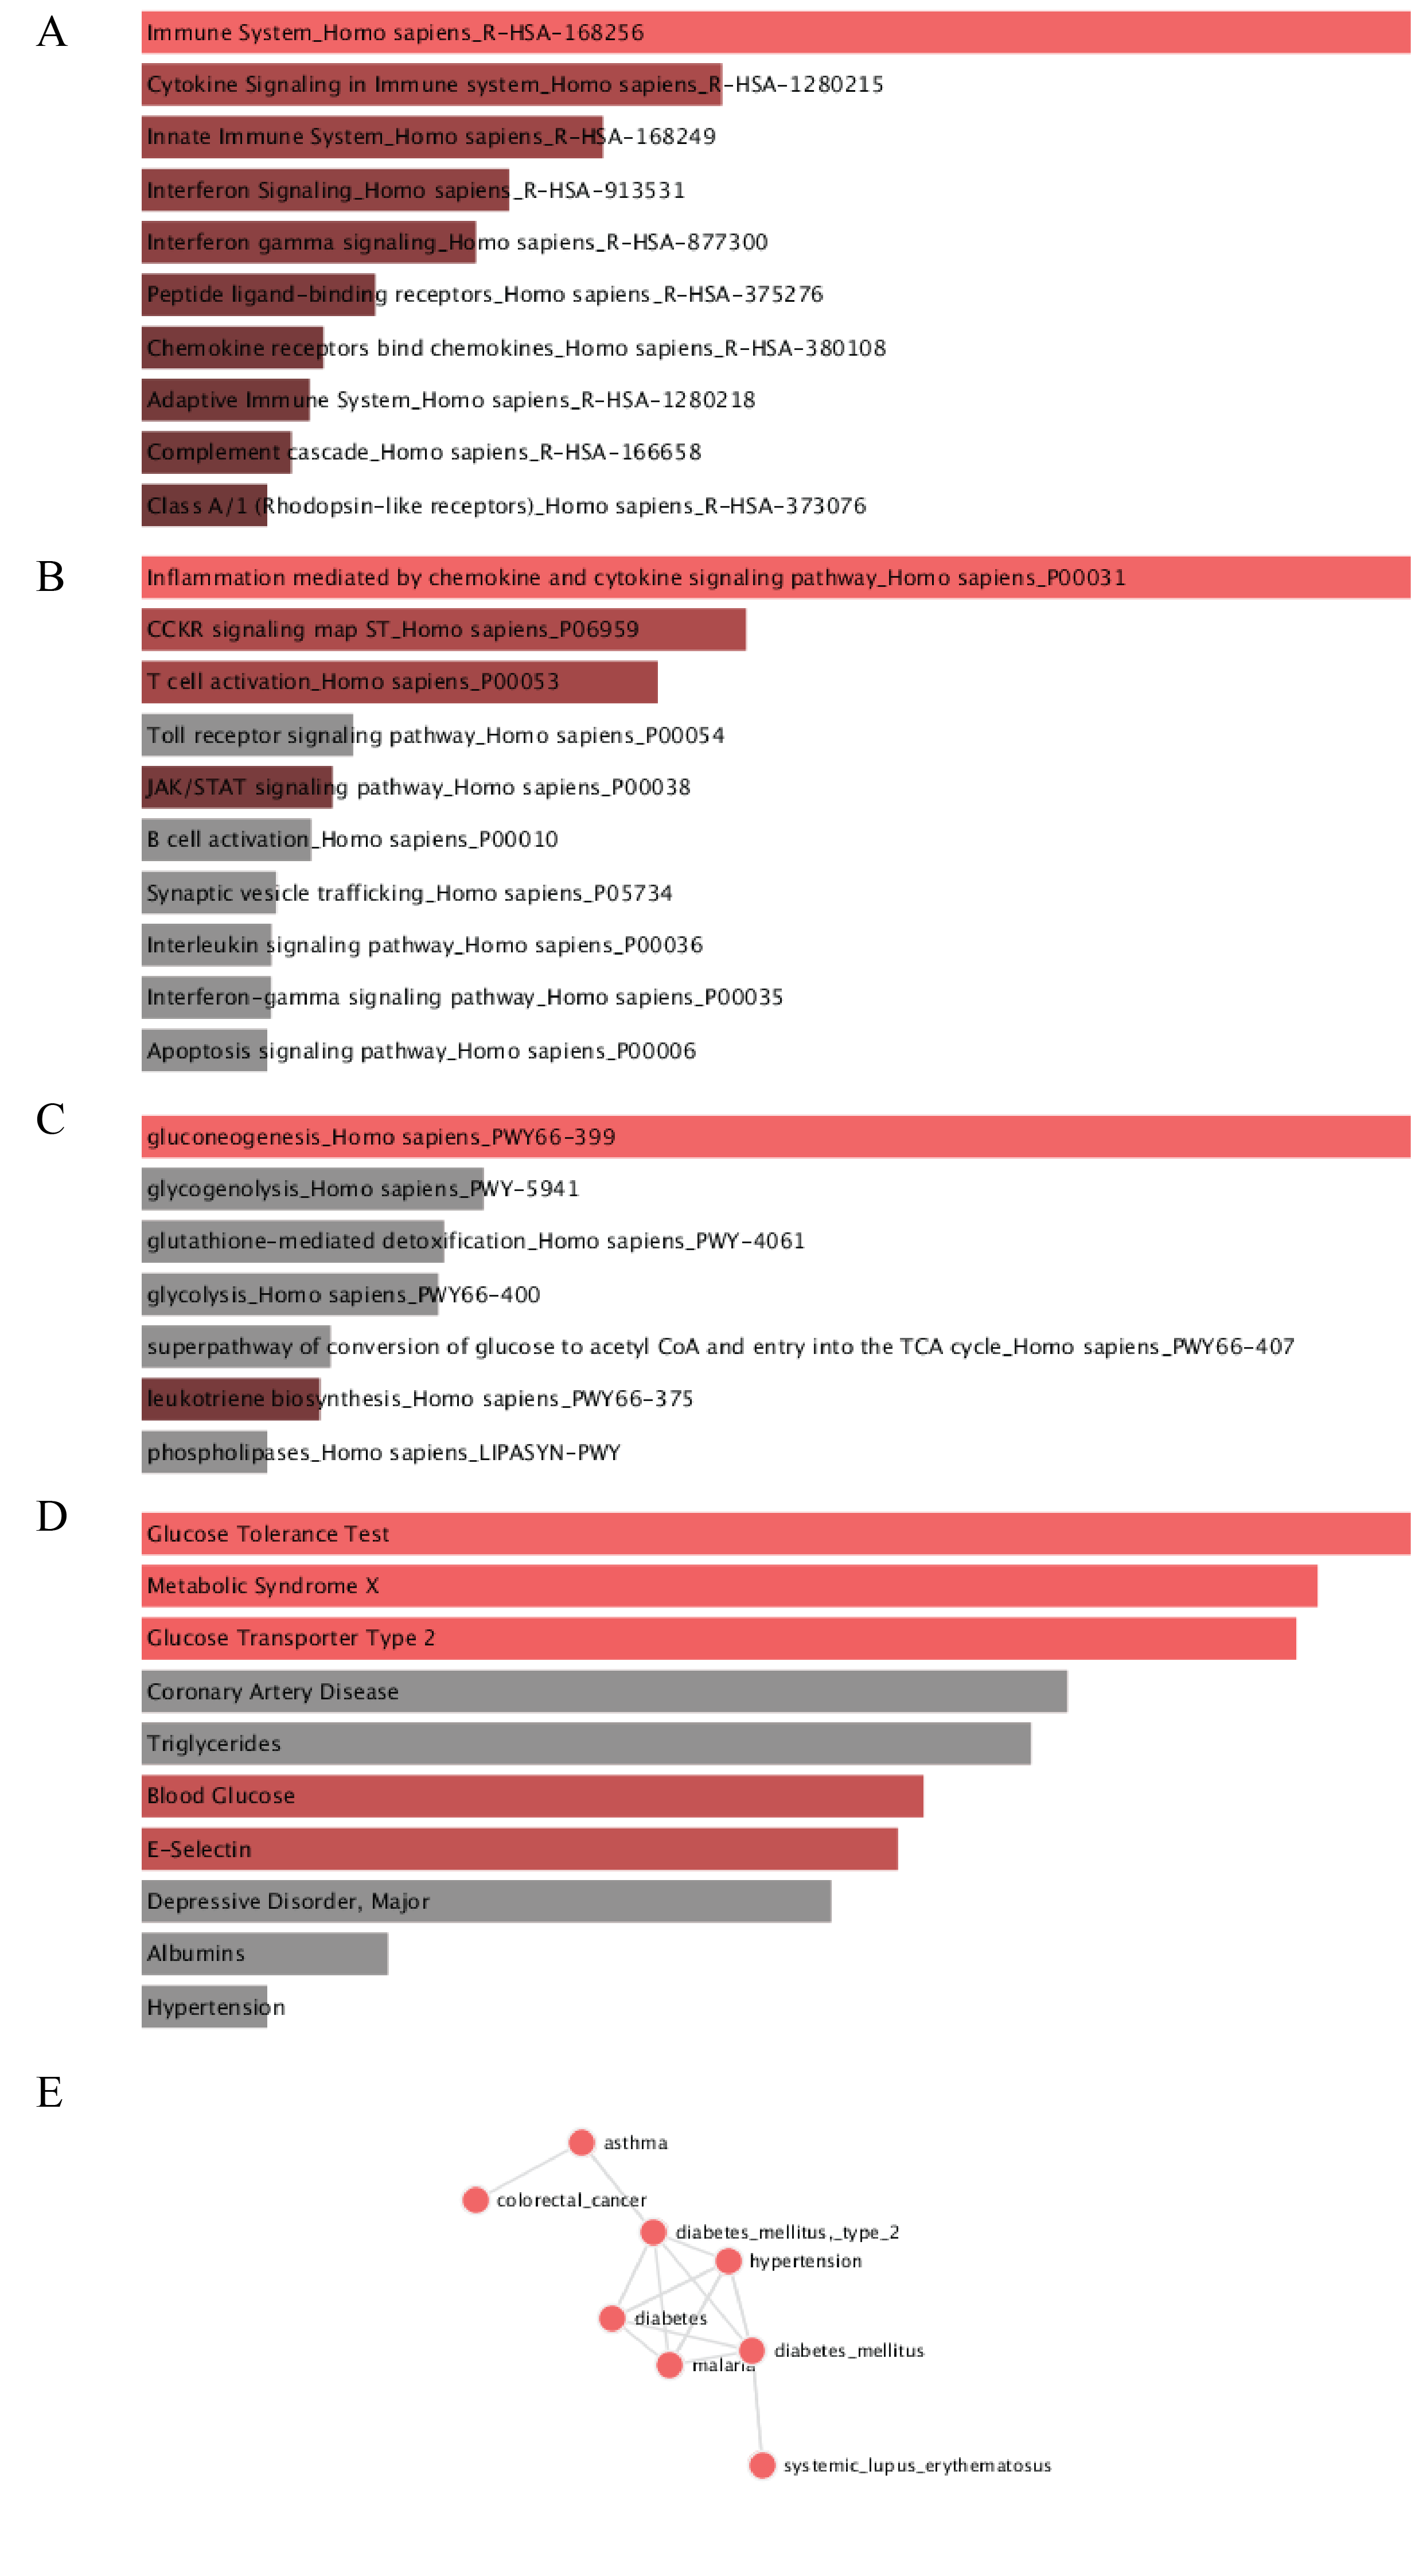
\includegraphics[width=\textwidth,height=\textheight,keepaspectratio]{GIM/figureS1.png}%Figure from images\Figure1.png
	\caption[Enrichment analysis of the type 1 diabetes genes.]{(Continued on the following page)}
	\label{fig:s0GIM}
\end{figure}
\begin{figure}[t]
  \contcaption{Enrichment analysis of the type 1 diabetes differentially expressed genes in A- Reactome and B-Panther database and the enrichment of the metabolic genes in C- the HumanCyc database, D- the dbGap database, and the E- OMIM database.}% Continued caption
\end{figure}
\subsection{Simulation setting} \label{GIM:spsim}
\subsubsection{Tolerance tests}
We used dHarvey to simulate the outcome of the different tolerance tests.
The kinetic parameters provided with the GIM model were used to represent the doses and time of intake. We applied the constraints dynamically on Harvey in each time step following the indirect coupling method. In IVGTT, where a dose of glucose is injected intravenously, we added an exchange reaction to represent the intake of glucose in the blood \textit{glc\_D[bc]} during the 15 mn of infusion (67.7 mmol/5mn). Consequently, we solved Harvey using pFBA \cite{lewis2010omic} assuming a whole-body maintenance objective function and aggregated the results in a matrix for each time step comprised of the tolerance tests in columns and the metabolic fluxes in rows. We reduced the matrix through PCA, and plotted the time-course of the first component (Figure \ref{fig:GIM1}-E) to illustrate the whole-body metabolic shift induced by a insulin and glucose tolerance tests. The points were fit on a 6\textsuperscript{th} order polynomial curve (Figure \ref{fig:GIM1}-E).\\
Furthermore, in order to assess if the dHarvey model was sensitive to the dynamical constraints applied from the GIM model, we aggregated the pFBA simulation results over 600 mn of simulation per 5mn time step. In each tolerance test simulation, we built a feature matrix comprised of the whole-body metabolic fluxes  in columns and the tolerance test in each time step in rows. With a time step of 5mn, 120 simulation result in T1D and healthy formed the 240 rows. We then reduced each matrix of the tolerance test using PCA. We took the 10 first component of the PCA, as they were significant at $p<0.001$. The component significance was assessed through 100 random permutation of the columns followed by PCA on the perturbed matrix. The 10 first component were then used as features in a binary SVM to classify healthy and T1D based on whole-body fluxes in each tolerance test. We used an SVM with a Gaussian kernel and performed 3-fold cross-validation on the training set (80\%) and predicted the labels of the test set (20\%). The data was standardized and the process was repeated 100 times taking every time a different partition of the training and test set.
We choose to use significant components as features instead of performing feature selection on the whole-body fluxes as the focus was the assessment of dHarvey sensitivity towards glucose and insulin challenges and the subsequent whole-body metabolic shift. The fluxes used in each time step are one among many possible solutions in the AOS space, and cannot be used as conclusive evidence on the disrupted metabolic pathways in T1D and healthy, even though pFBA reduces considerably the AOS space \cite{toroghi2016multi}. We addressed the question of disrupted  metabolic pathways in T1D through performing FVA in T1D and healthy models and using all the solution vectors of the AOS as a kernel for comparison. dHarvey was predictive towards T1D and healthy states in the tolerance tests (Figure (Figure \ref{fig:GIM1}-E), moreover when we used insulin and glucose challenges as classes in the SVM instead of T1D and healthy, whole-body fluxes were predictive towards them as well (Figure \ref{fig:s1GIM}). Taken together, dHarvey is predictive towards both the condition (T1D and healthy) and the perturbation (insulin and glucose challenges).
\begin{figure}[!htp]
\centering
	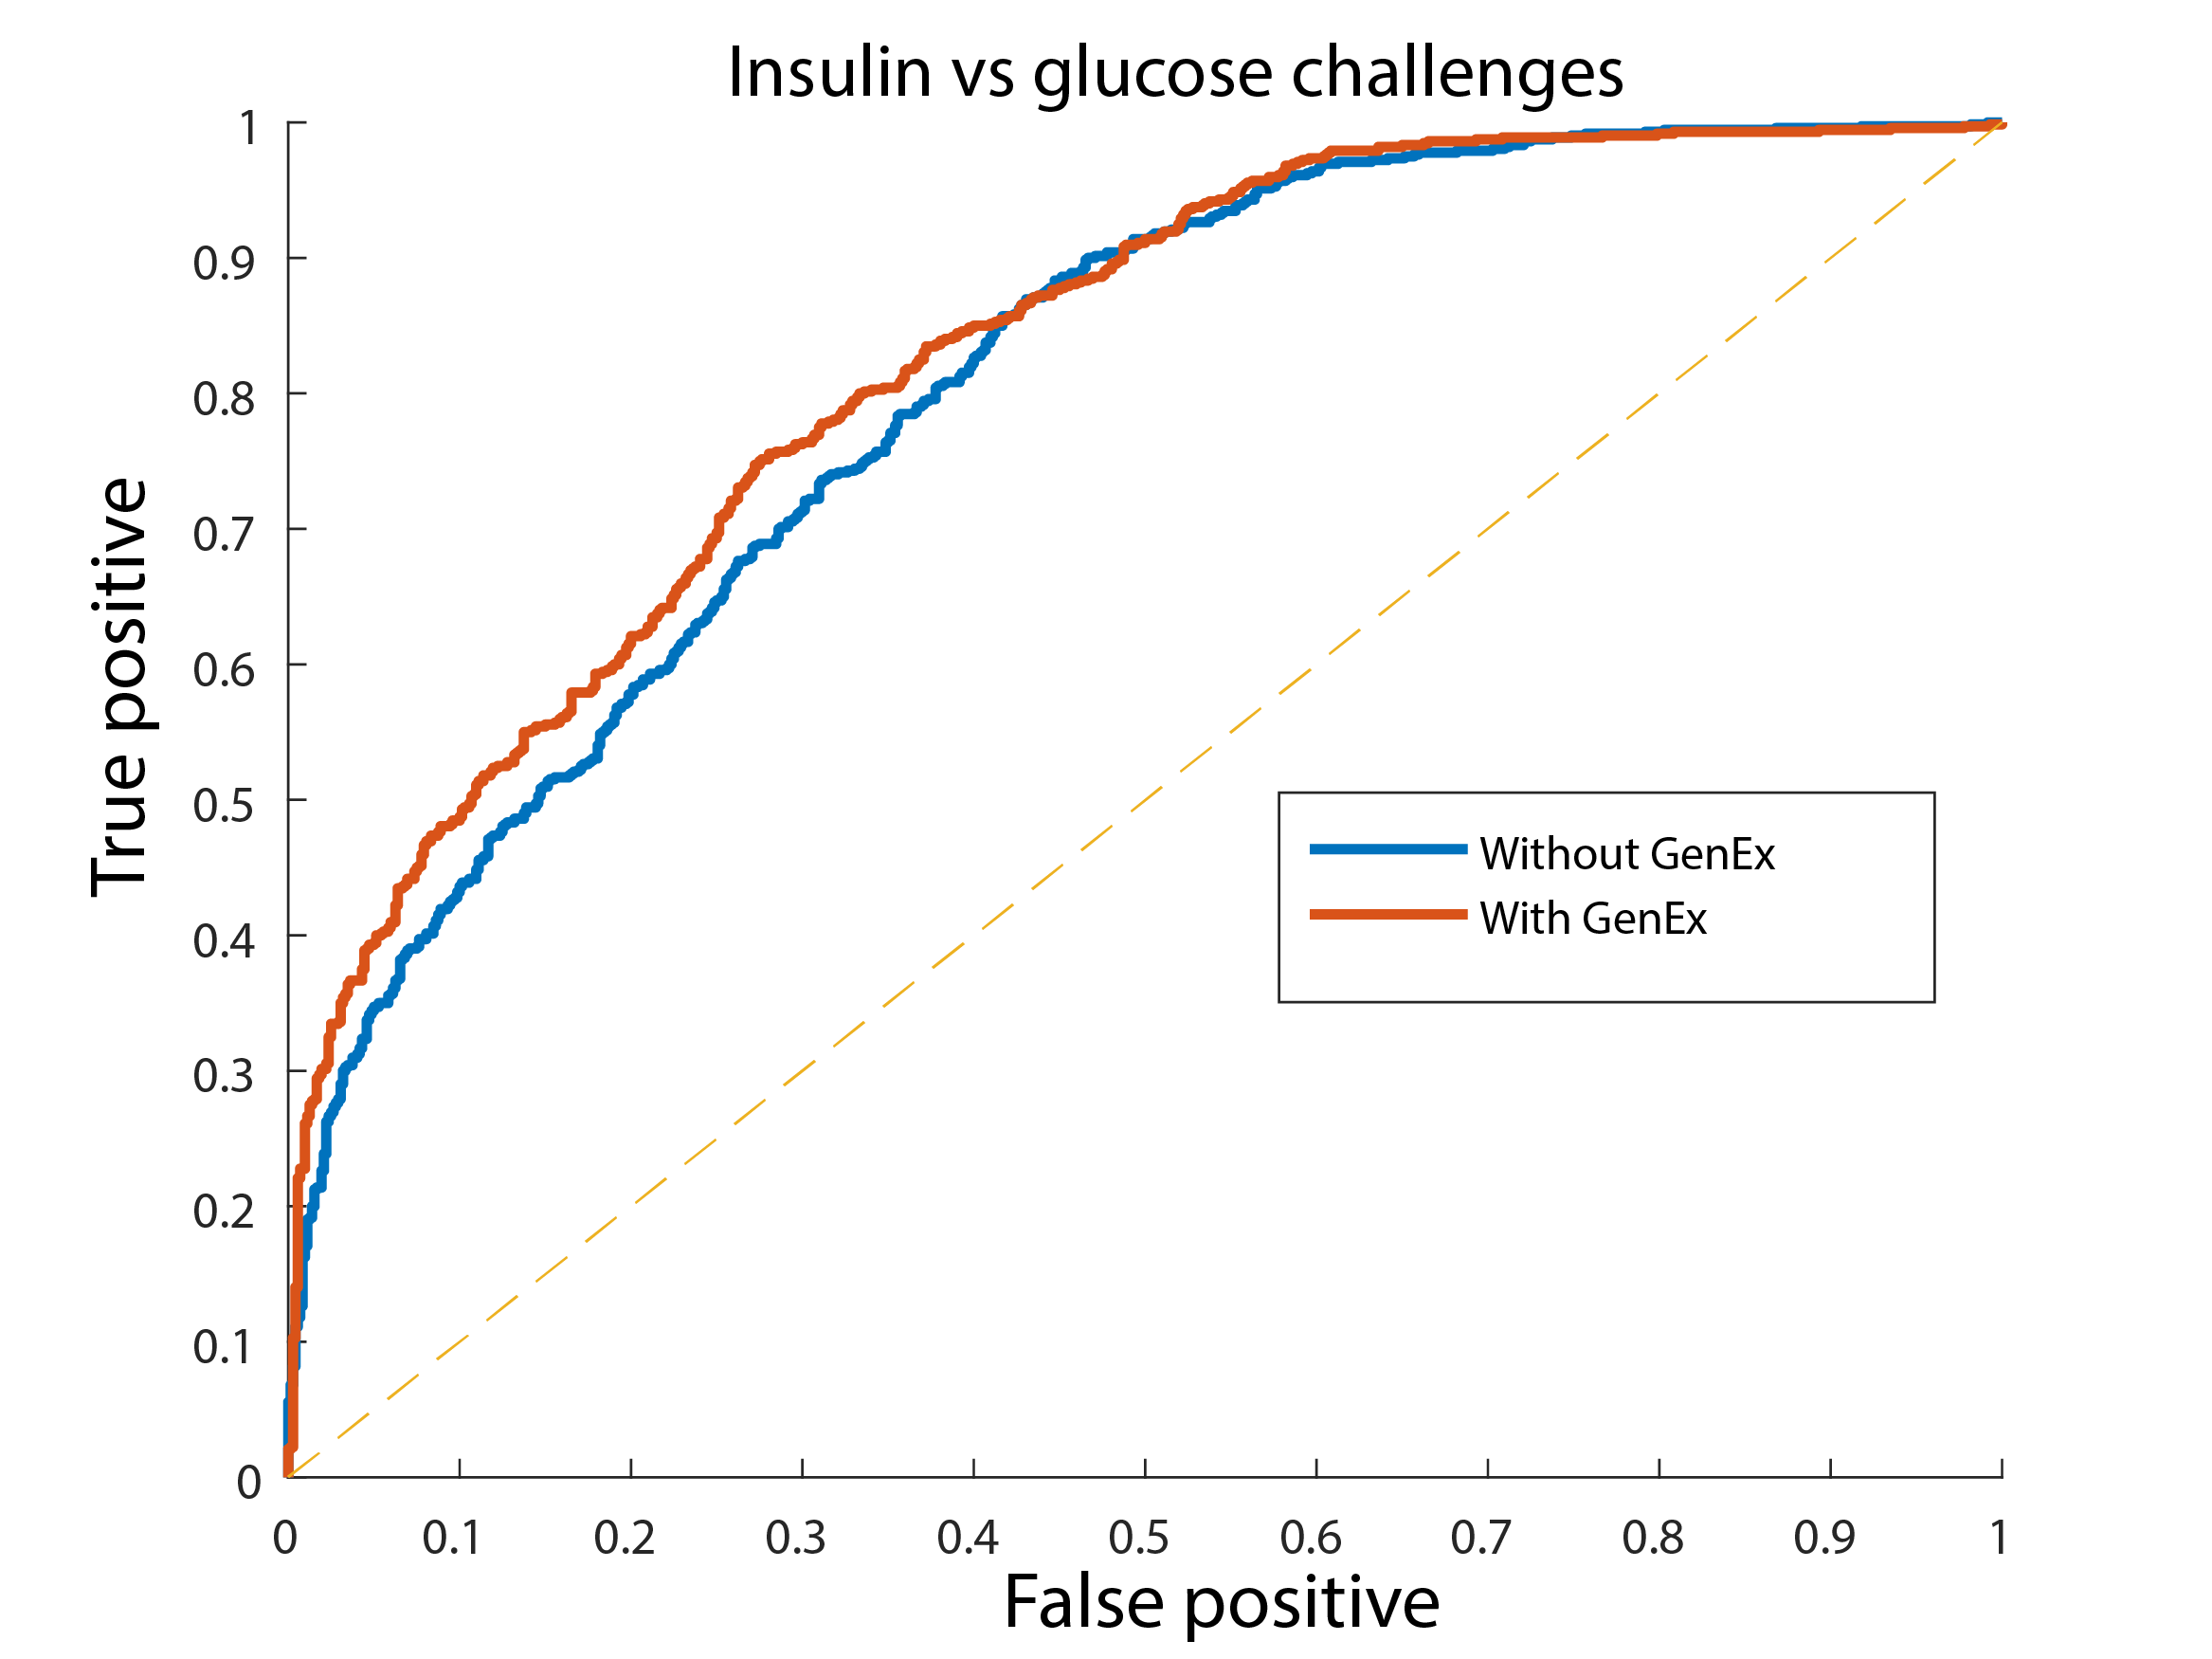
\includegraphics[width=\textwidth,height=\textheight,keepaspectratio]{GIM/figureSX.png}%Figure from images\Figure1.png
	\caption[Whole-body fluxes discriminate between insulin and glucose challenges.]{Whole-body fluxes discriminate between insulin and glucose challenges. A binary class support vectors machine accurately classifies insulin and glucose challenges using whole-body-fluxes. Constraining the model with T1D gene expression further improves the classification result. Insulin challenges were used as the true class.}
	\label{fig:s1GIM}
\end{figure}
\subsection{Relaxing infeasible problems} \label{GIM:sp2}
Subjecting dynamical model-derived constraints to the metabolic model could result in unfeasible problems. The situation could arise from conceptually different modeling approaches. In fact, the GIM model depicted short time events, while the constraint-based model was designed to simulate steady states. For instance, while it is commonly known that organs such as the lungs are glucose metabolizers rather than consumers, the GIM model could show a small secretion of glucose for a short time step as a consequence of free diffusion through the organ membrane. We relaxed the corresponding reactions in Harvey in order to obtain a feasible model through minimally relaxing the upper and lower bounds of the internal reactions. If the standard linear program is infeasible:\\
\begin{alignat*}{2} 
  & \text{max: } &  & c^{T}v\\
  & \text{subject to: } &  &  
                \begin{aligned}[t] \\
                & Sv=0 \\
                & v_{min} \leq v  \leq  v_{max}
                \end{aligned}
\end{alignat*}
, where $c^{T}.v$ is the objective function, $v$ is the flux vector of metabolic reactions, $c$ is the vector of objective coefficients, $S_{(m,n)}$ is the stoichiometric matrix linking $m$ metabolites and $n$ reactions, $lb$ is the vector of reaction lower bound, and $ub$ the vector of reaction upper bound. The following problem minimally relaxes the infeasible model:
\begin{alignat*}{2} 
  & \text{min: } &  & ||p||_{1},||q||_{1}\\
  & \text{subject to: } &  &  
                \begin{aligned}[t] \\
                & Sv=0 \\
                & v_{min} - p \leq v  \leq  v_{max} + q
                \end{aligned}
\end{alignat*}
,where $p$ is the relaxation vector of the lower bound and $q$ is the relaxation vector of the upper bound. Minimizing the 1-norm of $p$ and $q$ ensures both sparsity (minimal cardinal of reactions to be relaxed), with minimal total sum of relaxation amplitude.
\begin{figure}[!htp]
\centering
	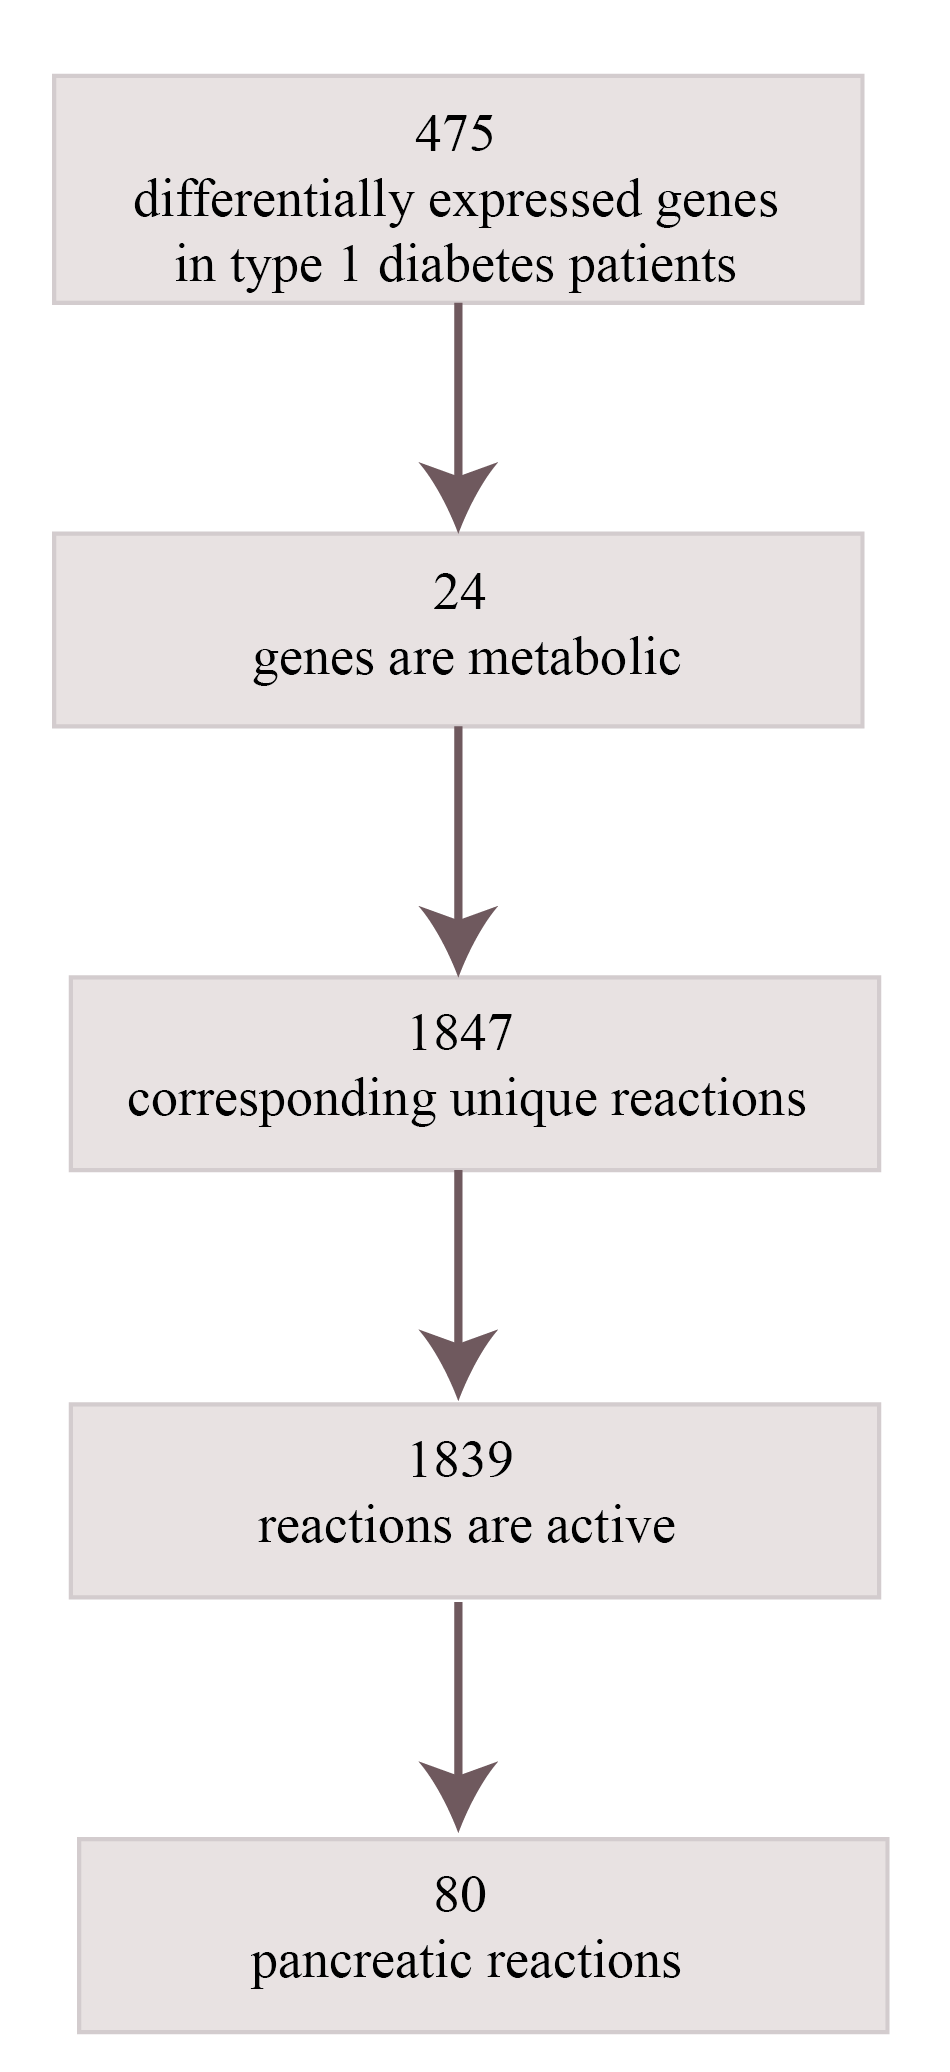
\includegraphics[width=\textwidth,height=\textheight,keepaspectratio]{GIM/figureS2.png}%Figure from images\Figure1.png
	\caption[Gene expression constraints pipeline.]{(Continued on the following page)}
	\label{fig:s2GIM}
\end{figure}
\begin{figure}[t]
  \contcaption{Gene expression constraints pipeline. The pancreas and pancreatic islets gene expression profile of type 1 diabetes patients \cite{planas2010gene} were translated into constraints. The reactions catalysed by a protein coded by a given gene are constrained by the lower and upper bound of gene expression fold change with respect to the control.}% Continued caption
\end{figure}
\subsection{CRONICS framework} \label{GIM:sp3}
The simulation of the hybrid model faced challenges related to 
\begin{itemize}
\item	The the size of the solution space in every time step and the effect of alternate optimal solutions, the problem being largely under-determined.  
\item	Also, the large size of the metabolic model required the reduction of the set of active reactions for subsequent analysis and biological interpretation. 
\item	Simulation time as a model would typically run in 2-3 days for 10 hours of simulation.
\end{itemize}
The above-mentioned challenges were addressed through combining a mosaic of existing techniques in the CRONICS framework which consists of the following steps:\\
\begin{enumerate}
\item	(optional) Depending on the simulation, the solution basis of the unconstrained problem is generated before coupling both the dynamical and metabolic model. The solution basis is then provided in all subsequent optimisation problems while activating the advanced start option in CPLEX as follows:\\
\begin{center}
ADVIND=1
\end{center}
\item	The setting starts with the simulation of dynamical model for 1 time step. Based on dFBA, The computed constraints are subjected to the metabolic model and a 1-norm minimal (pFBA) solution is selected given its sparse properties that allow for the selection of a smaller set of active reactions for further analysis.
\item	(Vertical coupling) The next time step in the dynamical model is simulated and the constraints are computed and subjected to the metabolic model. The selected solution is the one that is minimally distant to the previous solution (MOMA). This part allows to guarantee smoothness of the hybrid system, and the chronology of the simulation. Although the large size of the solution vector made the simulation computationally expensive, we chose a subset of the vector to minimize for. The minimal subset would be the coupled reactions themselves, in this case, the obtained vector is indeed nearly identical to the initial subset vector, which results in all simulations being converging to the dynamical model behaviour in terms of smoothness, while uncoupled reactions can be changing values abruptly in time steps as small as five minutes. While a subset containing reactions of the brain, liver, kidney, adipocytes, muscle, pancreas allowed to globally constrain the fluxes with respect to chronology of simulation while maintaining the smoothness of the system.
\item	(Horizontal coupling) In this previous setting the hybrid model consisted of a dynamically constrained metabolic network. In the horizontal setting, the dynamical model is in return constrained by the metabolic model. The obtained fluxes from the metabolic model serve as input for the next time step of the dynamical model. If the solution fluxes correspond to the input constraints then the hybrid model reaches the behaviour of the dynamical model alone. In both settings, the solution of the type 1 diabetes model in the first time step is minimally distant to the healthy model in the first time step.
\end{enumerate}
We used the CRONICS framework to predict metabolite concentrations in dHarvey model. The metabolites fell under two categories: the metabolites time-course predicted by GIM and the metabolites in Harvey that obey the steady-state assumption. Only the concentrations of imbalanced metabolites in Harvey can be predicted as they do not obey the steady-state assumption. We created demand reactions, which are imbalanced reactions, for metabolites of interest to predict the dynamic organ demand in these metabolites. We applied this method to predict the time-course of ATP demand in the liver (Figure \ref{fig:GIM2}-B), the triglyceride demand in the adipocytes (Figure \ref{fig:GIM3b}), and the valine and phenylalanine demand in plasma (Figure \ref{fig:GIM3a}).
\subsection{Software and solver parameters} \label{GIM:sp4}
The simulations were carried on MATLAB (2014b, Natick, MA, USA) with the ODE15s built-in function and with the COBRA toolbox v3.0 \cite{heirendt2017creation}  and the CPLEX and MAD TOMLAB v7.9 implementation on Windows 7 professional and ubuntu 16.04 –based high performance computing units.
The following parameters allowed a faster convergence as well as resolving ‘infeasbile after unscaling’ type of issues:\\
\begin{center}
PARALLEL=1\\
THREADS=2\\
SCAIND= -1\\
EPMRK=0.9 \\
NUMERICALEMPHASIS=1 \\
EPOPT=1e-6 \\
EPRHS=1e-6 \\
\end{center}
\subsection{Differentially expressed fluxes between healthy and type 1 diabetic models} \label{GIM:sp5}
\begin{figure}[!htp]
\centering
	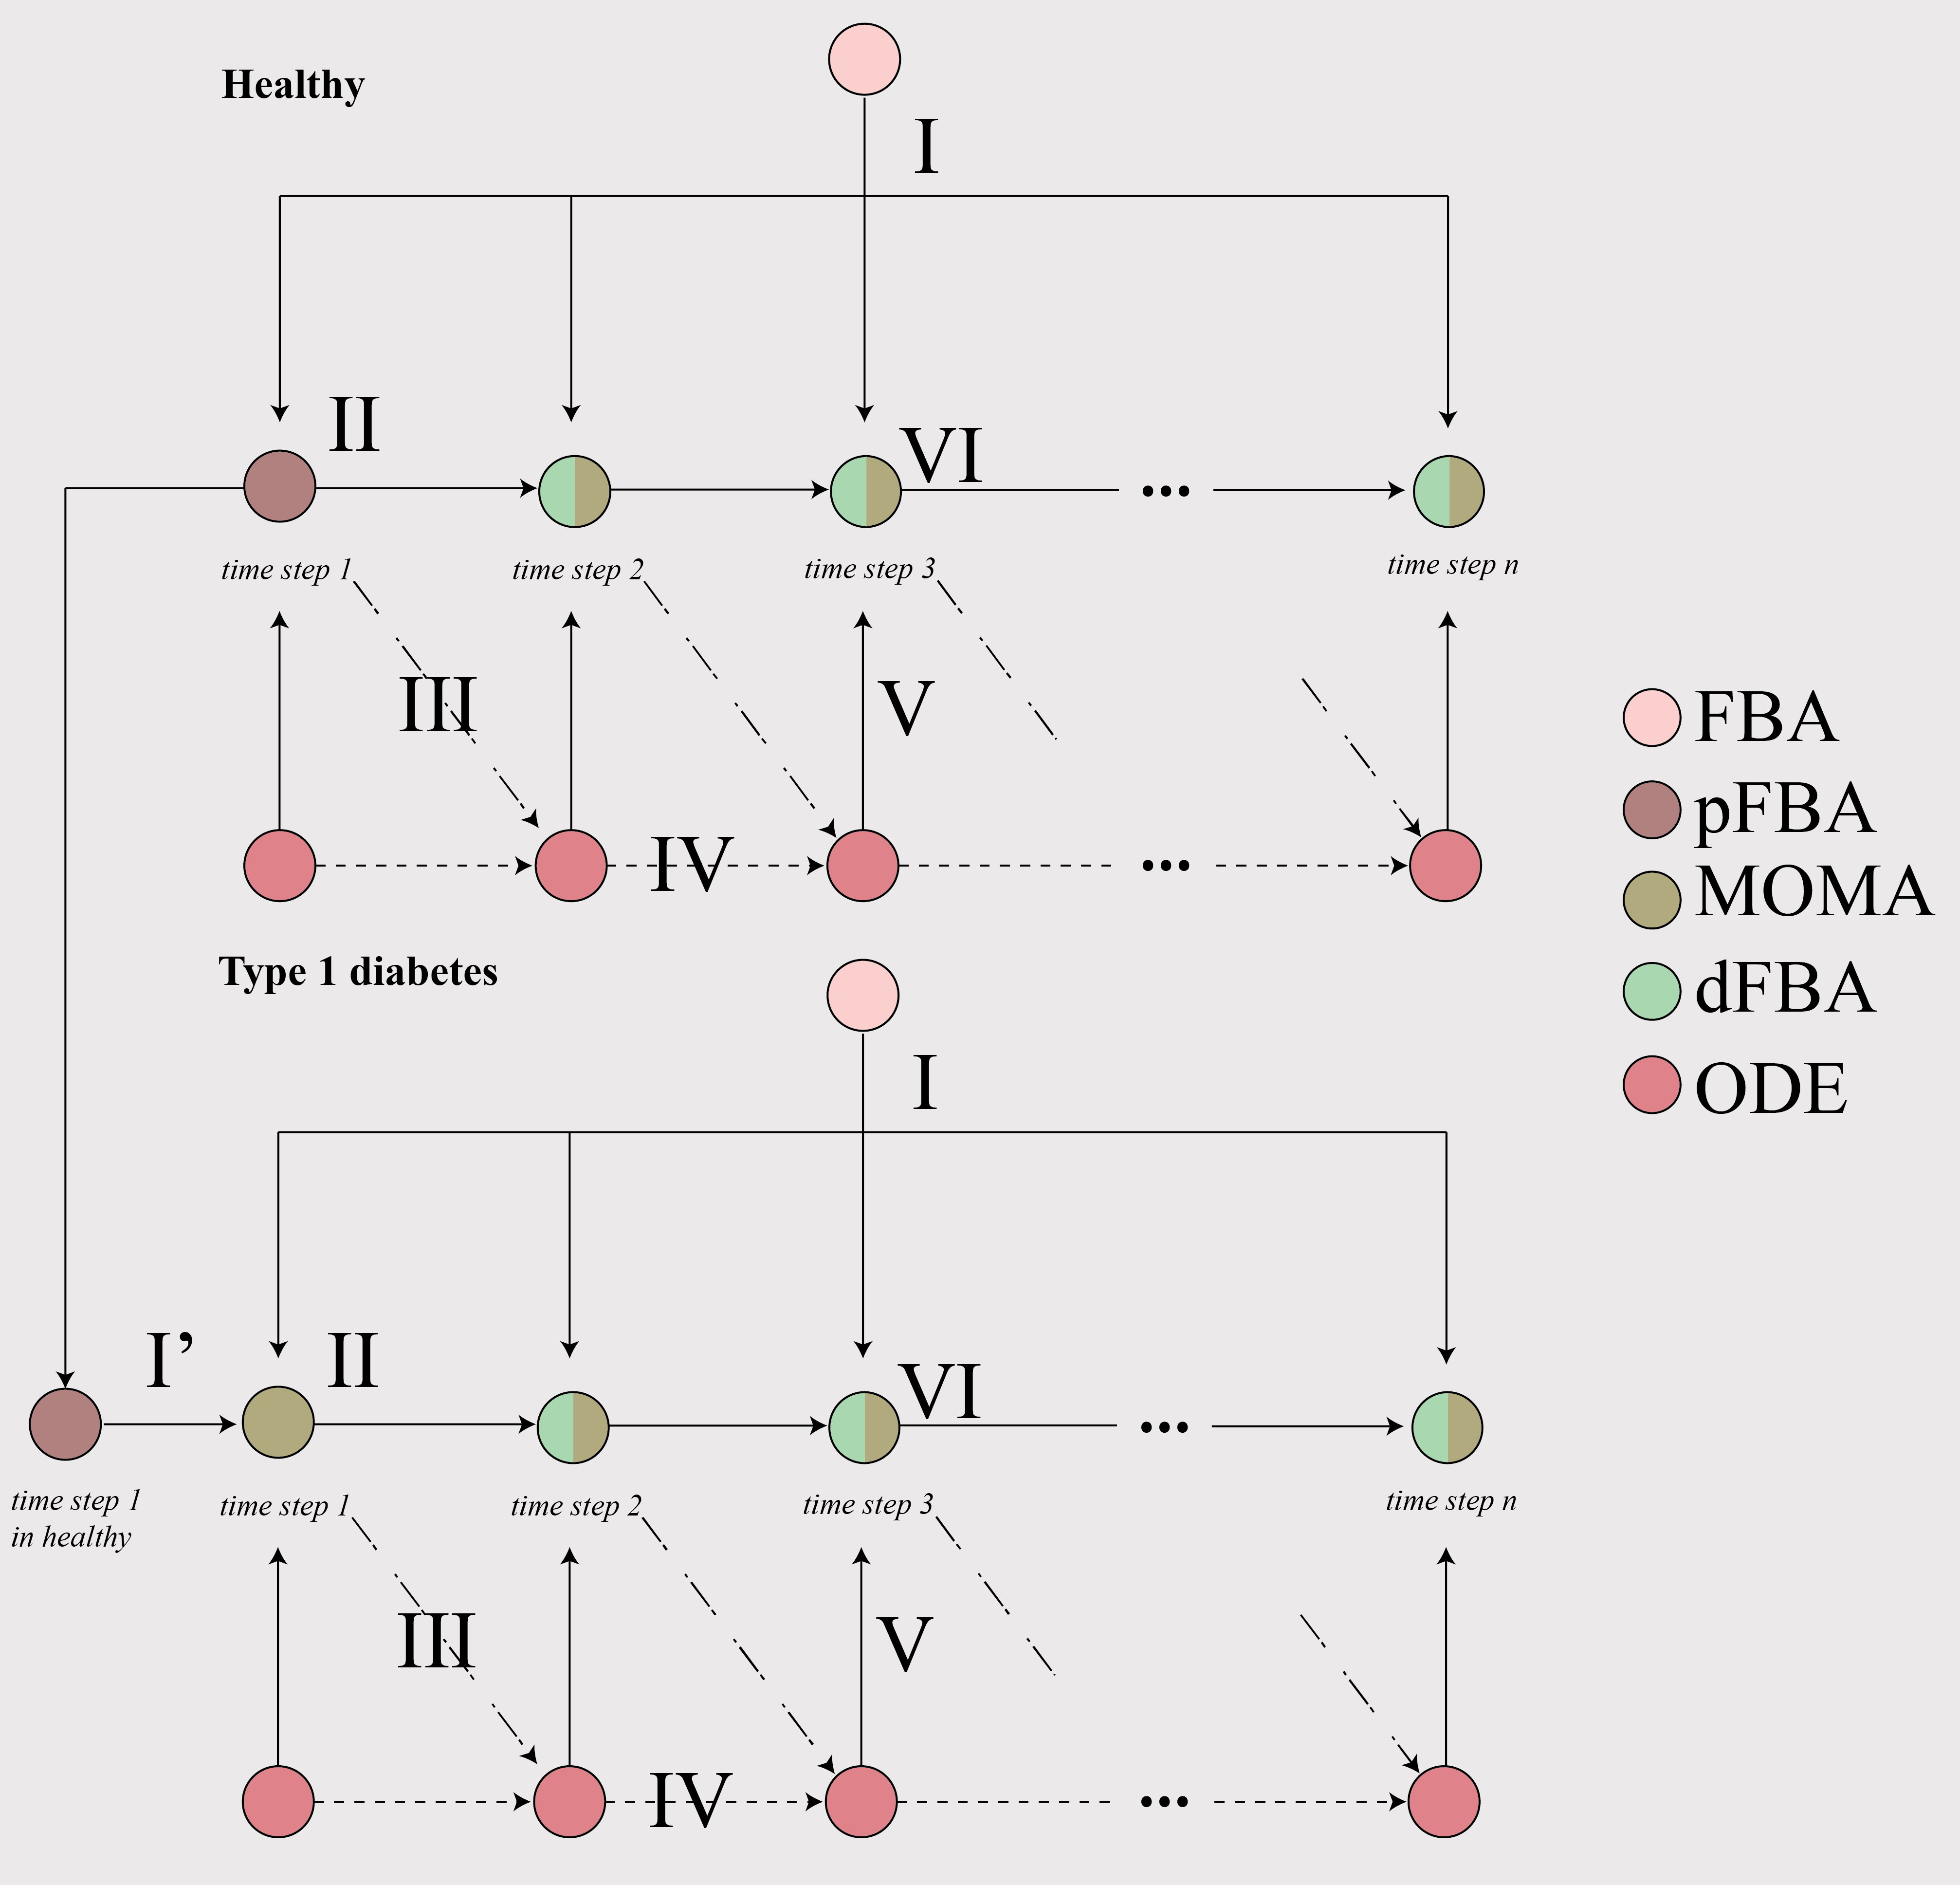
\includegraphics[width=\textwidth,height=\textheight,keepaspectratio]{GIM/figureS3.png}%Figure from images\Figure1.png
	\caption[CRONICS framework for dynamical simulation of genome scale models.]{CRONICS framework for dynamical simulation of genome scale models. The algorithm starts with solving the I) general unconstrained problem with FBA and using its solution basis as a warmstart for the next time steps. II) The first time step is then solved using pFBA after subjecting constraints from the dynamical model to ensure the sparsity of all subsequent solutions. Depending on the type of coupling, the algorithm would either use the constrained-based III) solution as initial estimate for the next time step of the dynamical model to obtain IV) new derivatives that will be subjected on the V) constrained-based model. Alternatively, the dynamical model is independent from the constraint-based model and feedback is only unidirectional (V but not III). The LP problem in the new time step will get constraints from the corresponding time step of the dynamical model, and VI) it will also be constrained by the previous time step so that solutions are minimally distant (MOMA). In type 1 diabetes, the first time step is further constrained by the first time step of the healthy model (I’), in order to ensure a minimal metabolic adjustment between the conditions. Initializing the simulations with pFBA solutions that are minimal to the healthy condition allows to propagate both the sparsity and the minimal metabolic adjustment to the healthy model to all the time steps. The CRONICS framework guarantees a smooth, continuous evolution of the system and reduces the effects of alternate optimal solutions on the predictions.}
	\label{fig:s3GIM}
\end{figure}
In order to compare the fluxes in both healthy and type 1 diabetic model, individual fluxes' comparison would yield inaccurate results given the large alternative optimal solution space. We compared flux distributions per reaction rather than the value provided by one solution. In order to obtain flux probability distributions, we performed flux variability analysis on both healthy and type 1 diabetic model. The COBRA toolbox function \textit{fastFVA} \cite{gudmundsson2010computationally} was called with the solutions as an output as following:\\
\begin{center} 
\textit{{[}minFluxH,maxFluxH,optsolH,retH,fbasolH,fvaminH,fvamaxH{]}=fastFVA(harveyIrrev,\\90,'max','cplex',harvey.rxns,'A',cpxControl)} \\
\end{center}
Prior to the flux variability analysis, the metabolic model was translated to its irreversible version, such as every reversible reaction is decomposed in the forward and the backward reaction, in a way that fluxes obtained are positive. The conversion was done using the following COBRA toolbox function:\\
\begin{center}
\textit{{[}harveyIrrev,matchRev,rev2irrev,irrev2rev{]}
=convertToIrreversibleCoupled(harvey)}\\
\end{center}
The obtained flux distribution per reactions equalled 160320 sample per reaction (80160 reaction* 2 (minimization and maximization)). The two matrices containing the fluxes values per reaction in healthy and type 1 diabetic model were used as an input to volcano plot function \textit{mavolcanoplot} in MATLAB (2014b, Natick, MA, USA). A p-value less than 0.001 was considered as a significance threshold for a minimal fold change of 1.3. Higher values of fold change are usually used in gene expression experiments, with the objective of containing small value change that is related to the experimental set up among several factors. As these considerations do not apply to linear programs solutions, provided the same solver settings, we considered a smaller fold change value.
\subsection{Enrichment of gene vectors}
After obtaining the up-regulated and down-regulated fluxes in T1D, we connected the reactions to their encoding genes and performed gene set enrichment analysis. The set of obtained genes would correspond experimentally to the differentially expressed genes and we queried i) the LINCS database to look for small molecules that reverse the signature of T1D, meaning the compound that induce a reverse genetic signature to the T1D signature that we obtained, which can potentially reverse the metabolic profile and ii) we queried the KEGG database to assess which disease were similar in signature to T1D.\\
In order to determine potential small molecules that can reverse T1D, we collected the list of up-regulated and down-regulated genes in T1D and queried the LINCS Canvas Browser \cite{duan2014lincs}, setting the up-regulated genes and down-regulated genes in the up and down field respectively and using the \textit{reverse} option to look for small molecule that reverse the queried signature. The results are reported in table \ref{GIM:tbls6}.\\
To determine the diseases that have a similar genetic signature to T1D, we merged the up-regulated and down-regulated reactions into a unique set of differentially expressed reactions. Since one metabolic reaction can be encoded by one or more genes using boolean operations (AND, OR), there can be several genetic profiles corresponding to a single metabolic profile. We randomly selected 10,000 genetic profile corresponding to the metabolic profile of T1D and queried each one of them programmatically in Enrichr \cite{chen2013enrichr} through the API. Subsequently, we selected the top five most enriched terms in the KEGG database at p<0.05 for each of the 10,000 gene profiles. Then we ranked the terms by their occurrence in each profile (Figure \ref{fig:sx2GIM}). An example of the output of the enrichment of one profile is listed in table \ref{GIM:tbls5}.\\
The enrichment of metabolic reactions in organs and subsystems as groups was done through a one-sided hypergeometric test with FDR correction. 
%The results are in//metabolic disease PD AD
\begin{figure}[!htp]
\centering
	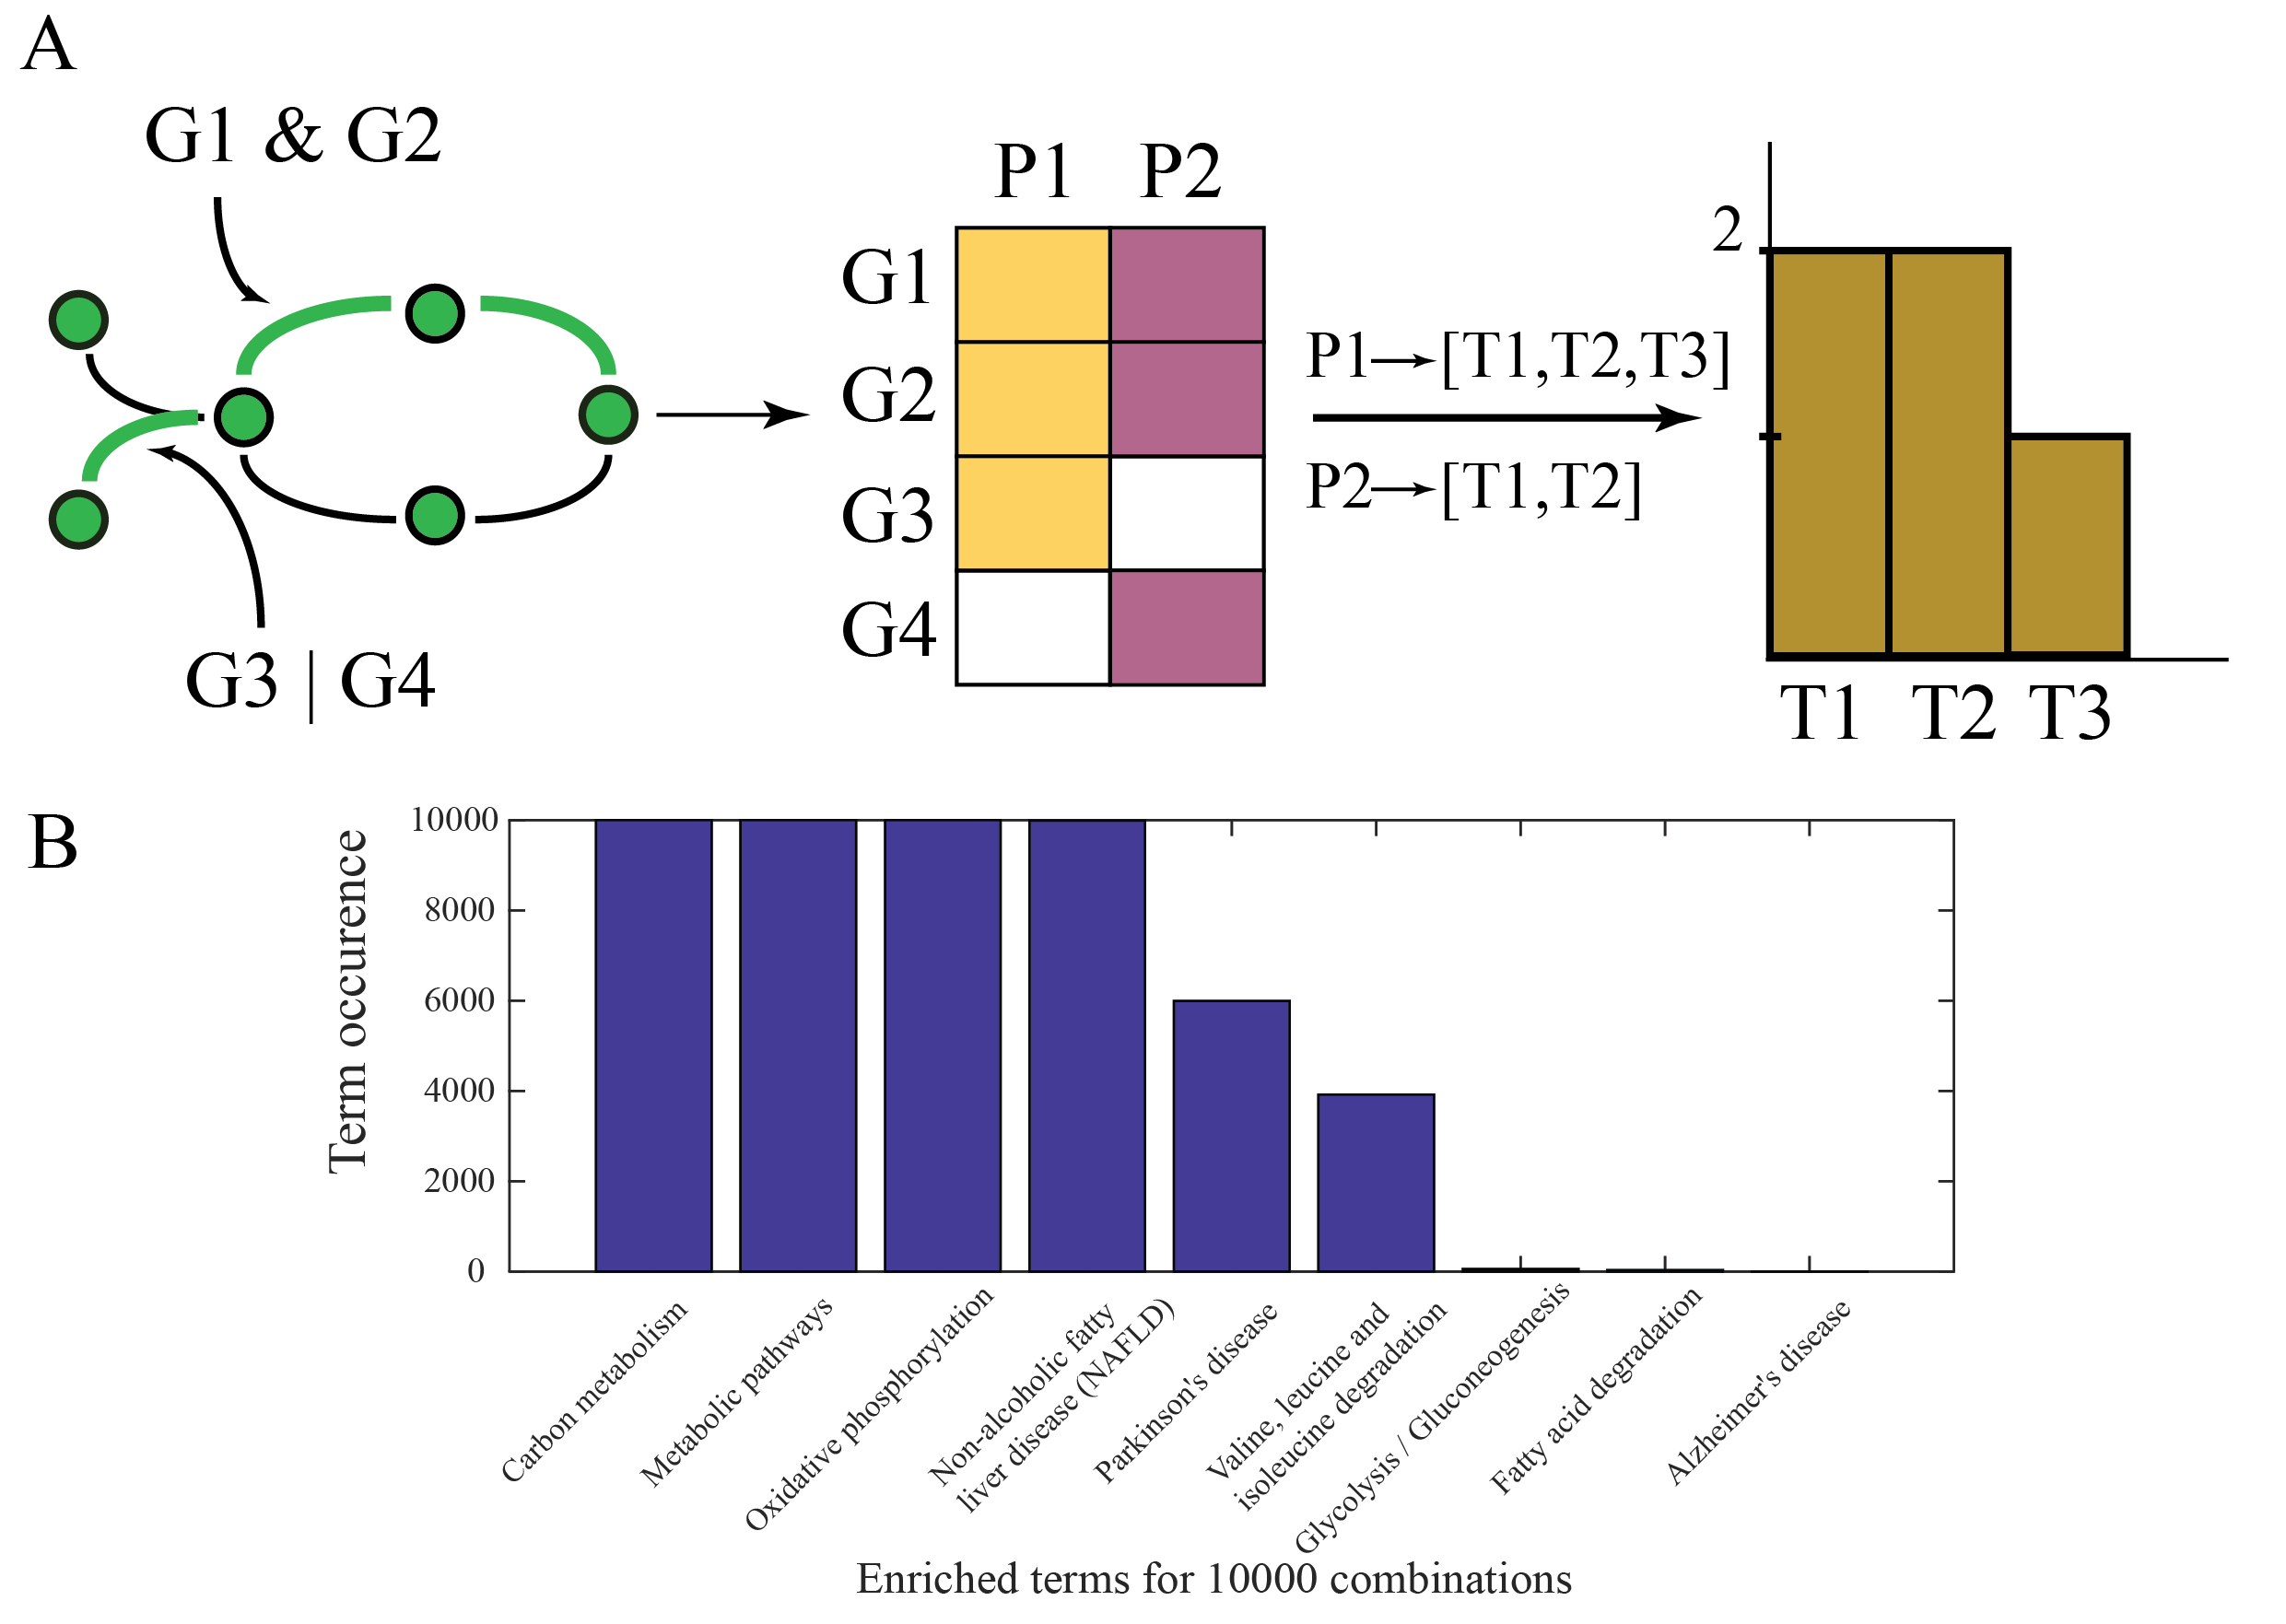
\includegraphics[width=\textwidth,height=\textheight,keepaspectratio]{GIM/figureSX2.png}%Figure from images\Figure1.png
	\caption[Enrichment of gene expression profiles in KEGG.]{Enrichment of gene expression profiles in KEGG. A- The process of deriving gene profile form metabolic profiles and B- its application to T1D. The identification of differential reaction fluxes in T1D allows to link back to the encoding genes. Since several genes can encode for the same reaction through AND, OR rules in the metabolic model, there can be several differential gene (G) profiles corresponding to one metabolic profile. We sampled 10000 profiles corresponding to the T1D profile and queried KEGG through Enrichr \cite{chen2013enrichr} for each of the profiles (P). The enriched terms (T) for each profile were classified by their occurrence in the 10000 profiles.}
	\label{fig:sx2GIM}
\end{figure}
\subsection{Comparison of flux density estimates}
In order to determine the metabolic effects of insulin in T1D (Figure \ref{fig:GIM3}), we first computed the alternate optimal solutions in T1D model prior to insulin injection, using FVA. We obtained 160032 solutions of the AOS of T1D model, which gives us as many number of flux values per reaction. Using the empirical flux values per reactions, we estimated the smoothed probability density function for each reaction. In a similar fashion, we collected solutions from the T1D model after the SCIB trial and equally, we estimated the probability density of flux values for each reaction. Finally, both density estimates were overlaid in order to compare the effect of insulin on the selection of flux values per enzyme/reaction.
\subsection{Intra-individual variability to insulin response}
We modelled the inter-individual variability to insulin response as the variation of kinetic parameters in GIM model. Consequently, We created 31 GIM model and coupled them to Harvey. The glucose concentrations are completely determined by the GIM model, also referred to as indirect coupling \cite{krauss2012integrating}.\\
Modeling the intra-individual variability to insulin consisted of using the average patient kinetic parameters in GIM and the variation of the internal state of the system as represented by Harvey. In this case, we randomly selected 1\% of reactions in every subsystem in every organ which resulted in a set of 2817 reactions that equally represented all the metabolic subsystems in all the organs. We assigned each reaction a random objective weight which corresponded to a metabolic state. Consequently, we created 31 metabolic state and simulated the models after the subcutaneous injection of insulin. Glucose concentrations are depend on both Harvey and GIM, also referred to as direct coupling \cite{krauss2012integrating}. The input matrix $X_{p,q}$ represents the objective coefficients of each of the $q$ reactions in the $p$ metabolic states. Here, $p=31$ and $q=2817$. The output matrix $Y_{p,n}$ represents the glucose concentrations at each of the $n$ time steps in the $p$ metabolic states, with $n=234$ with a 2.5 minutes time step length and the infusion starting at 16 minutes, totalling 10 hours of simulation. Using multivariate regression, we estimated the matrix $\rho_{q,n}$ that represents the sensitivities of each of the $q$ reactions towards each of the $n$ time steps of the simulation. In particular, the time steps corresponding to the minimal concentration $C_{min}$ and the final concentration $C_{final}$ were considered for further analysis, as they would link to hyperglycaemia and hypoglycaemia and diabetes control in general. The estimation of the sensitivity matrix consisted of solving the following equation:
\begin{gather*}
X* \rho \approx Y \\
\end{gather*}
We used the \textit{mvregress} routine in MATLAB and the Covariance Weighted Least Square (CWLS) algorithm to estimate $\rho$. The algorithm gives $p$ coefficients corresponding to $p$ out of $q$ reactions, wherein the rest in set to zero.
\begin{figure}[!htp]
\centering
	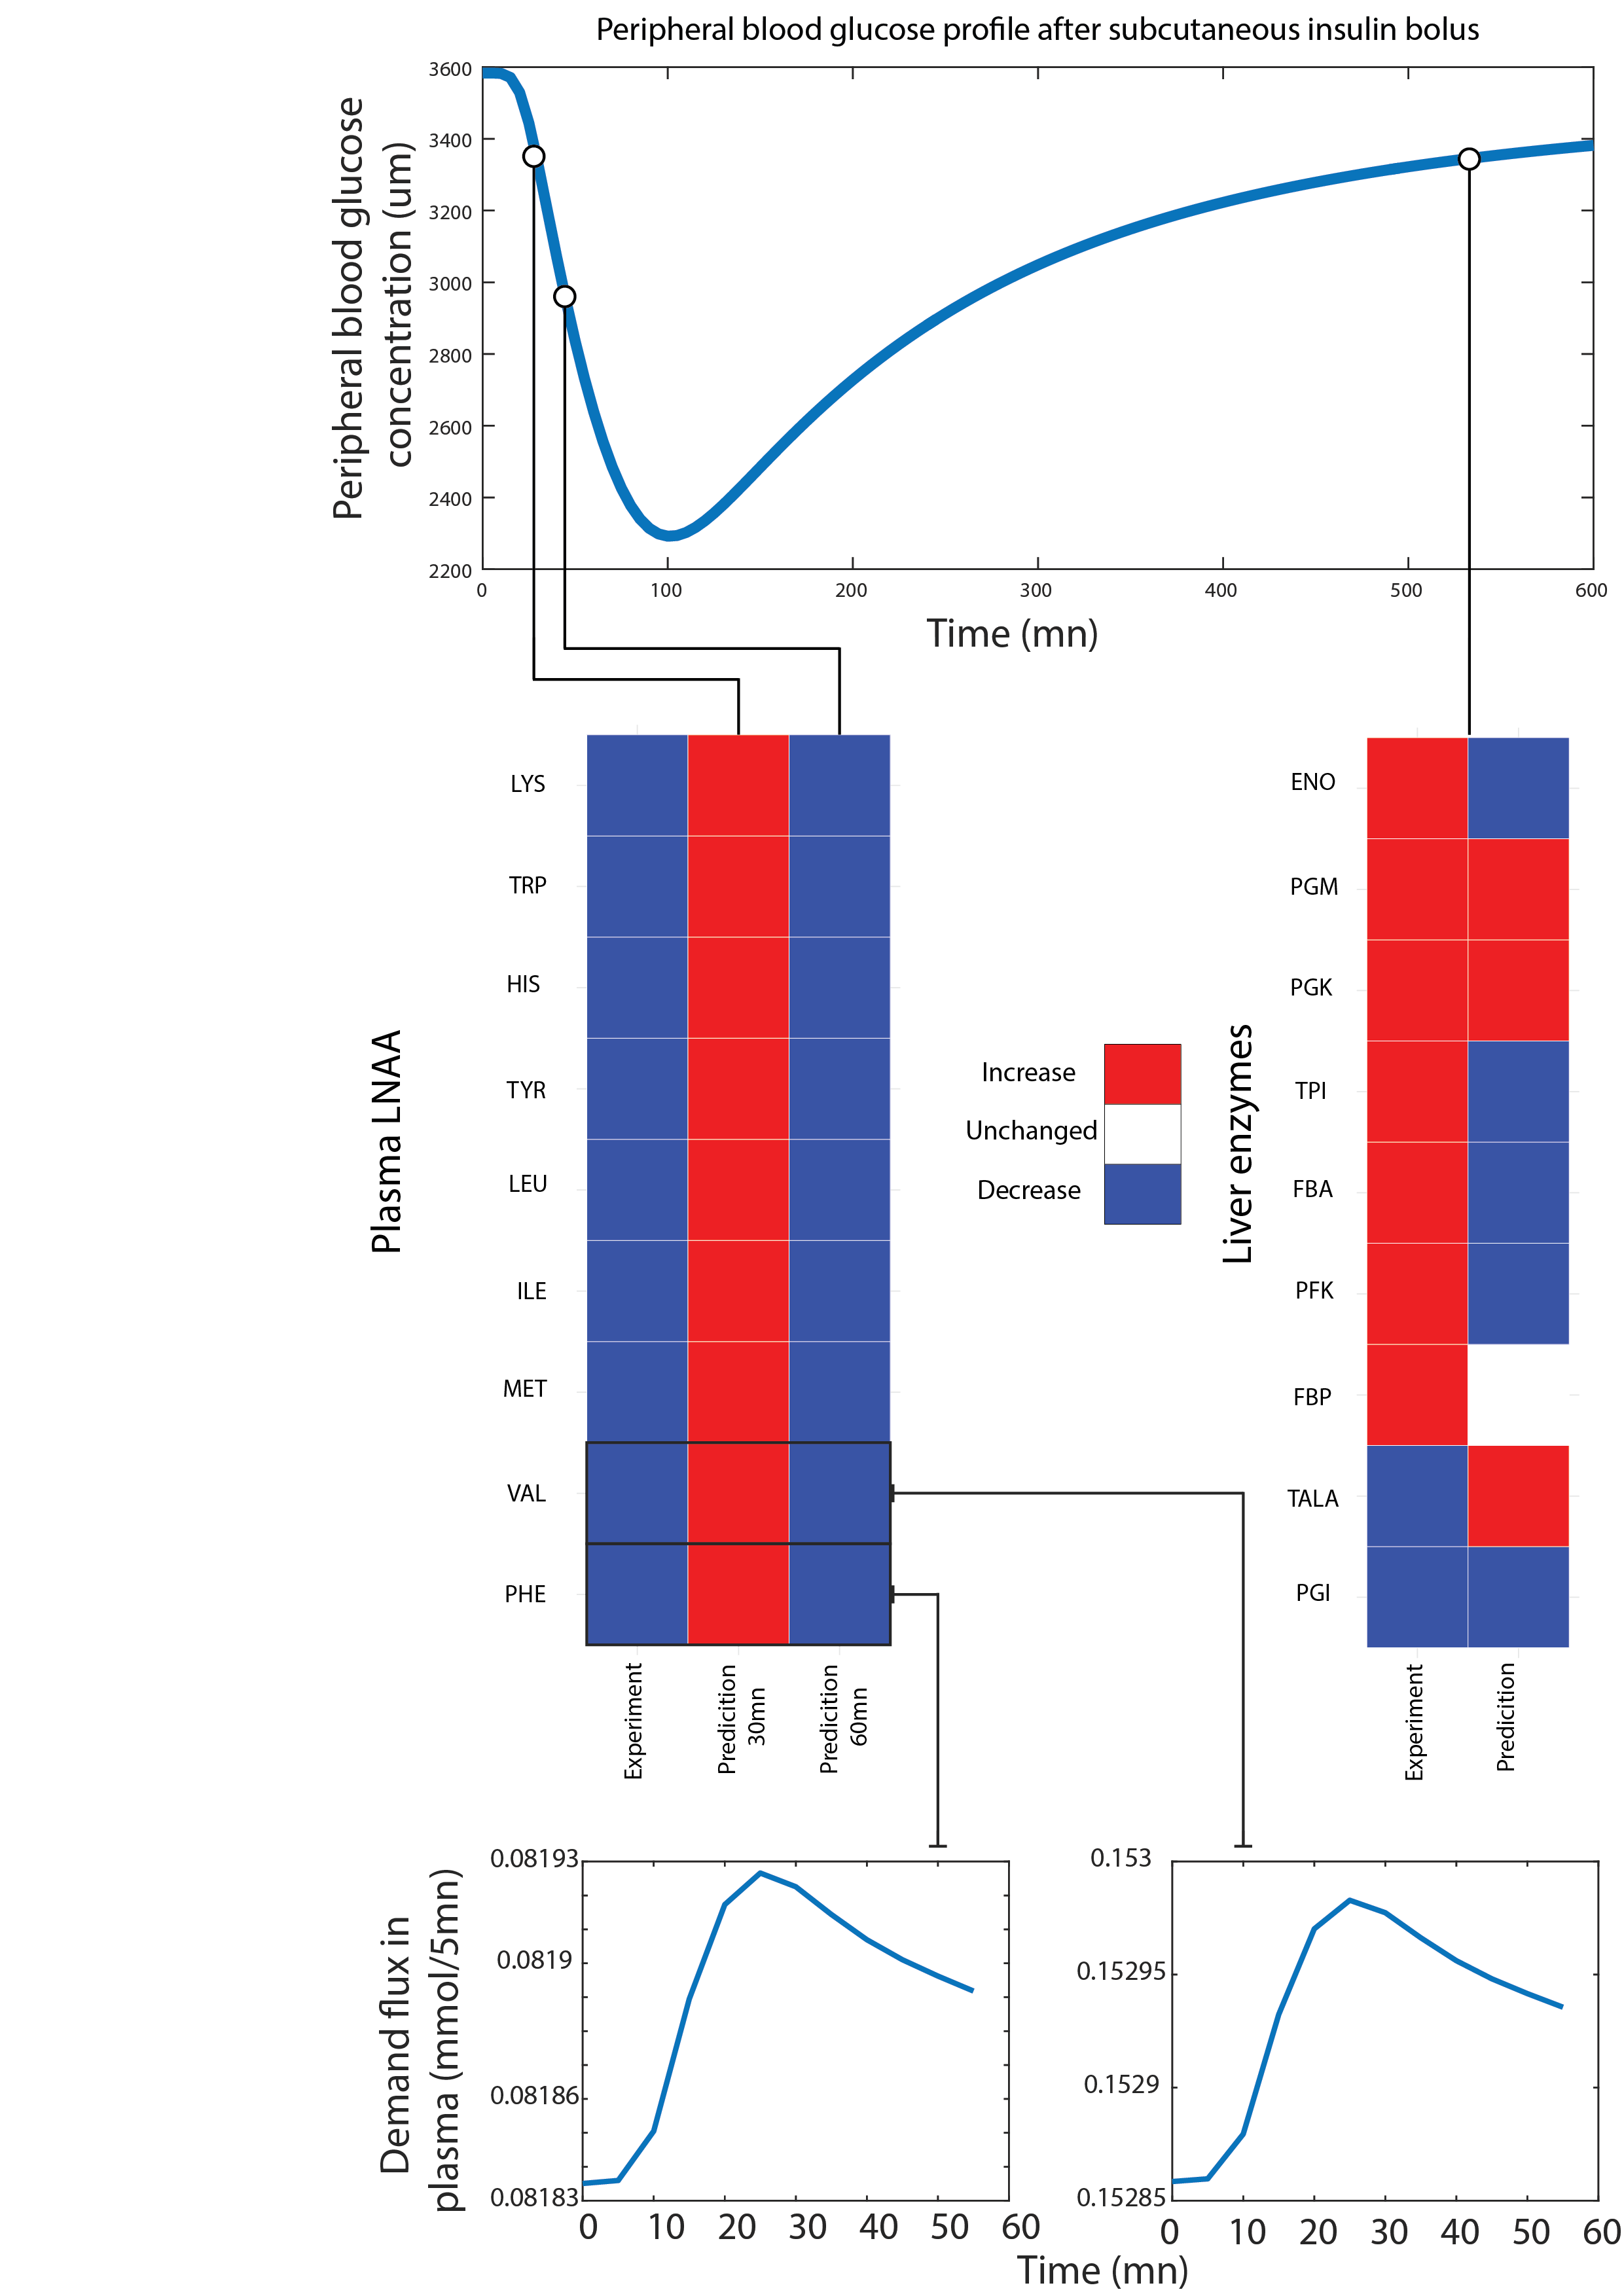
\includegraphics[width=\textwidth,height=\textheight,keepaspectratio]{GIM/figure3a.png}%Figure from images\Figure1.png
	\caption[Effect of insulin on LNAA concentrations.]{Predicted off-target effects on liver glycolytic enzymes and plasma large and neutral amino acids concentration (LNAA) after insulin subcutaneous administration.}
	\label{fig:GIM3a}
\end{figure}

\begin{figure}[!htp]
\centering
	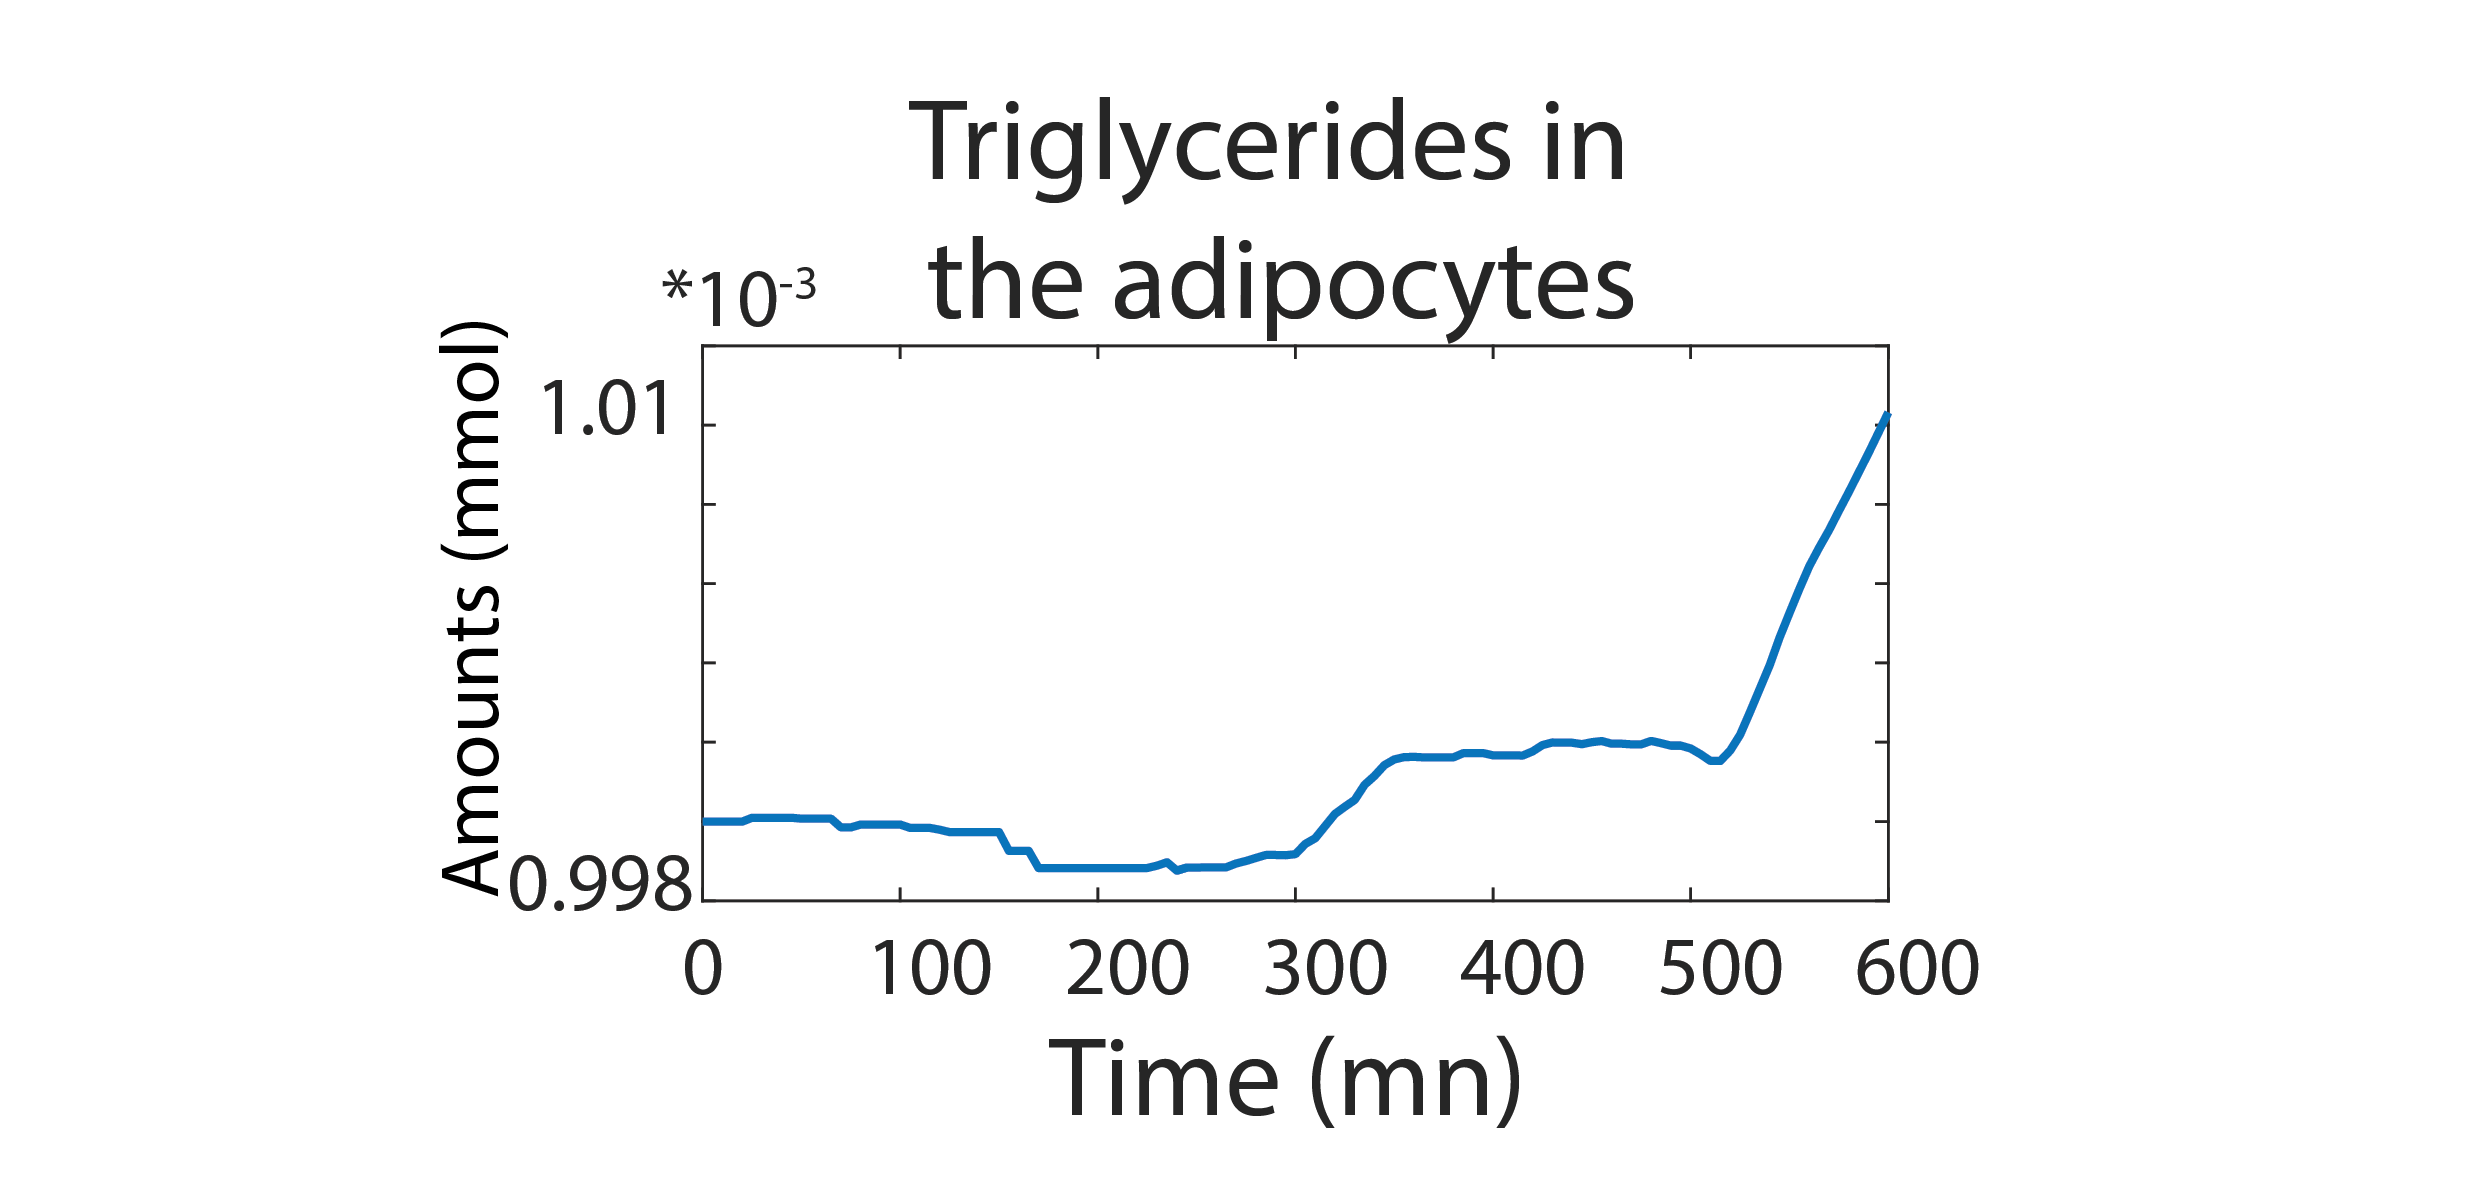
\includegraphics[width=\textwidth,height=\textheight,keepaspectratio]{GIM/TGdynamics.png}%Figure from images\Figure1.png
	\caption[Time-course of triglycerides in the adipocytes.]{Time-course of triglycerides in the adipocyte.}
	\label{fig:GIM3b}
\end{figure}

\begin{figure}[!htp]
\centering
	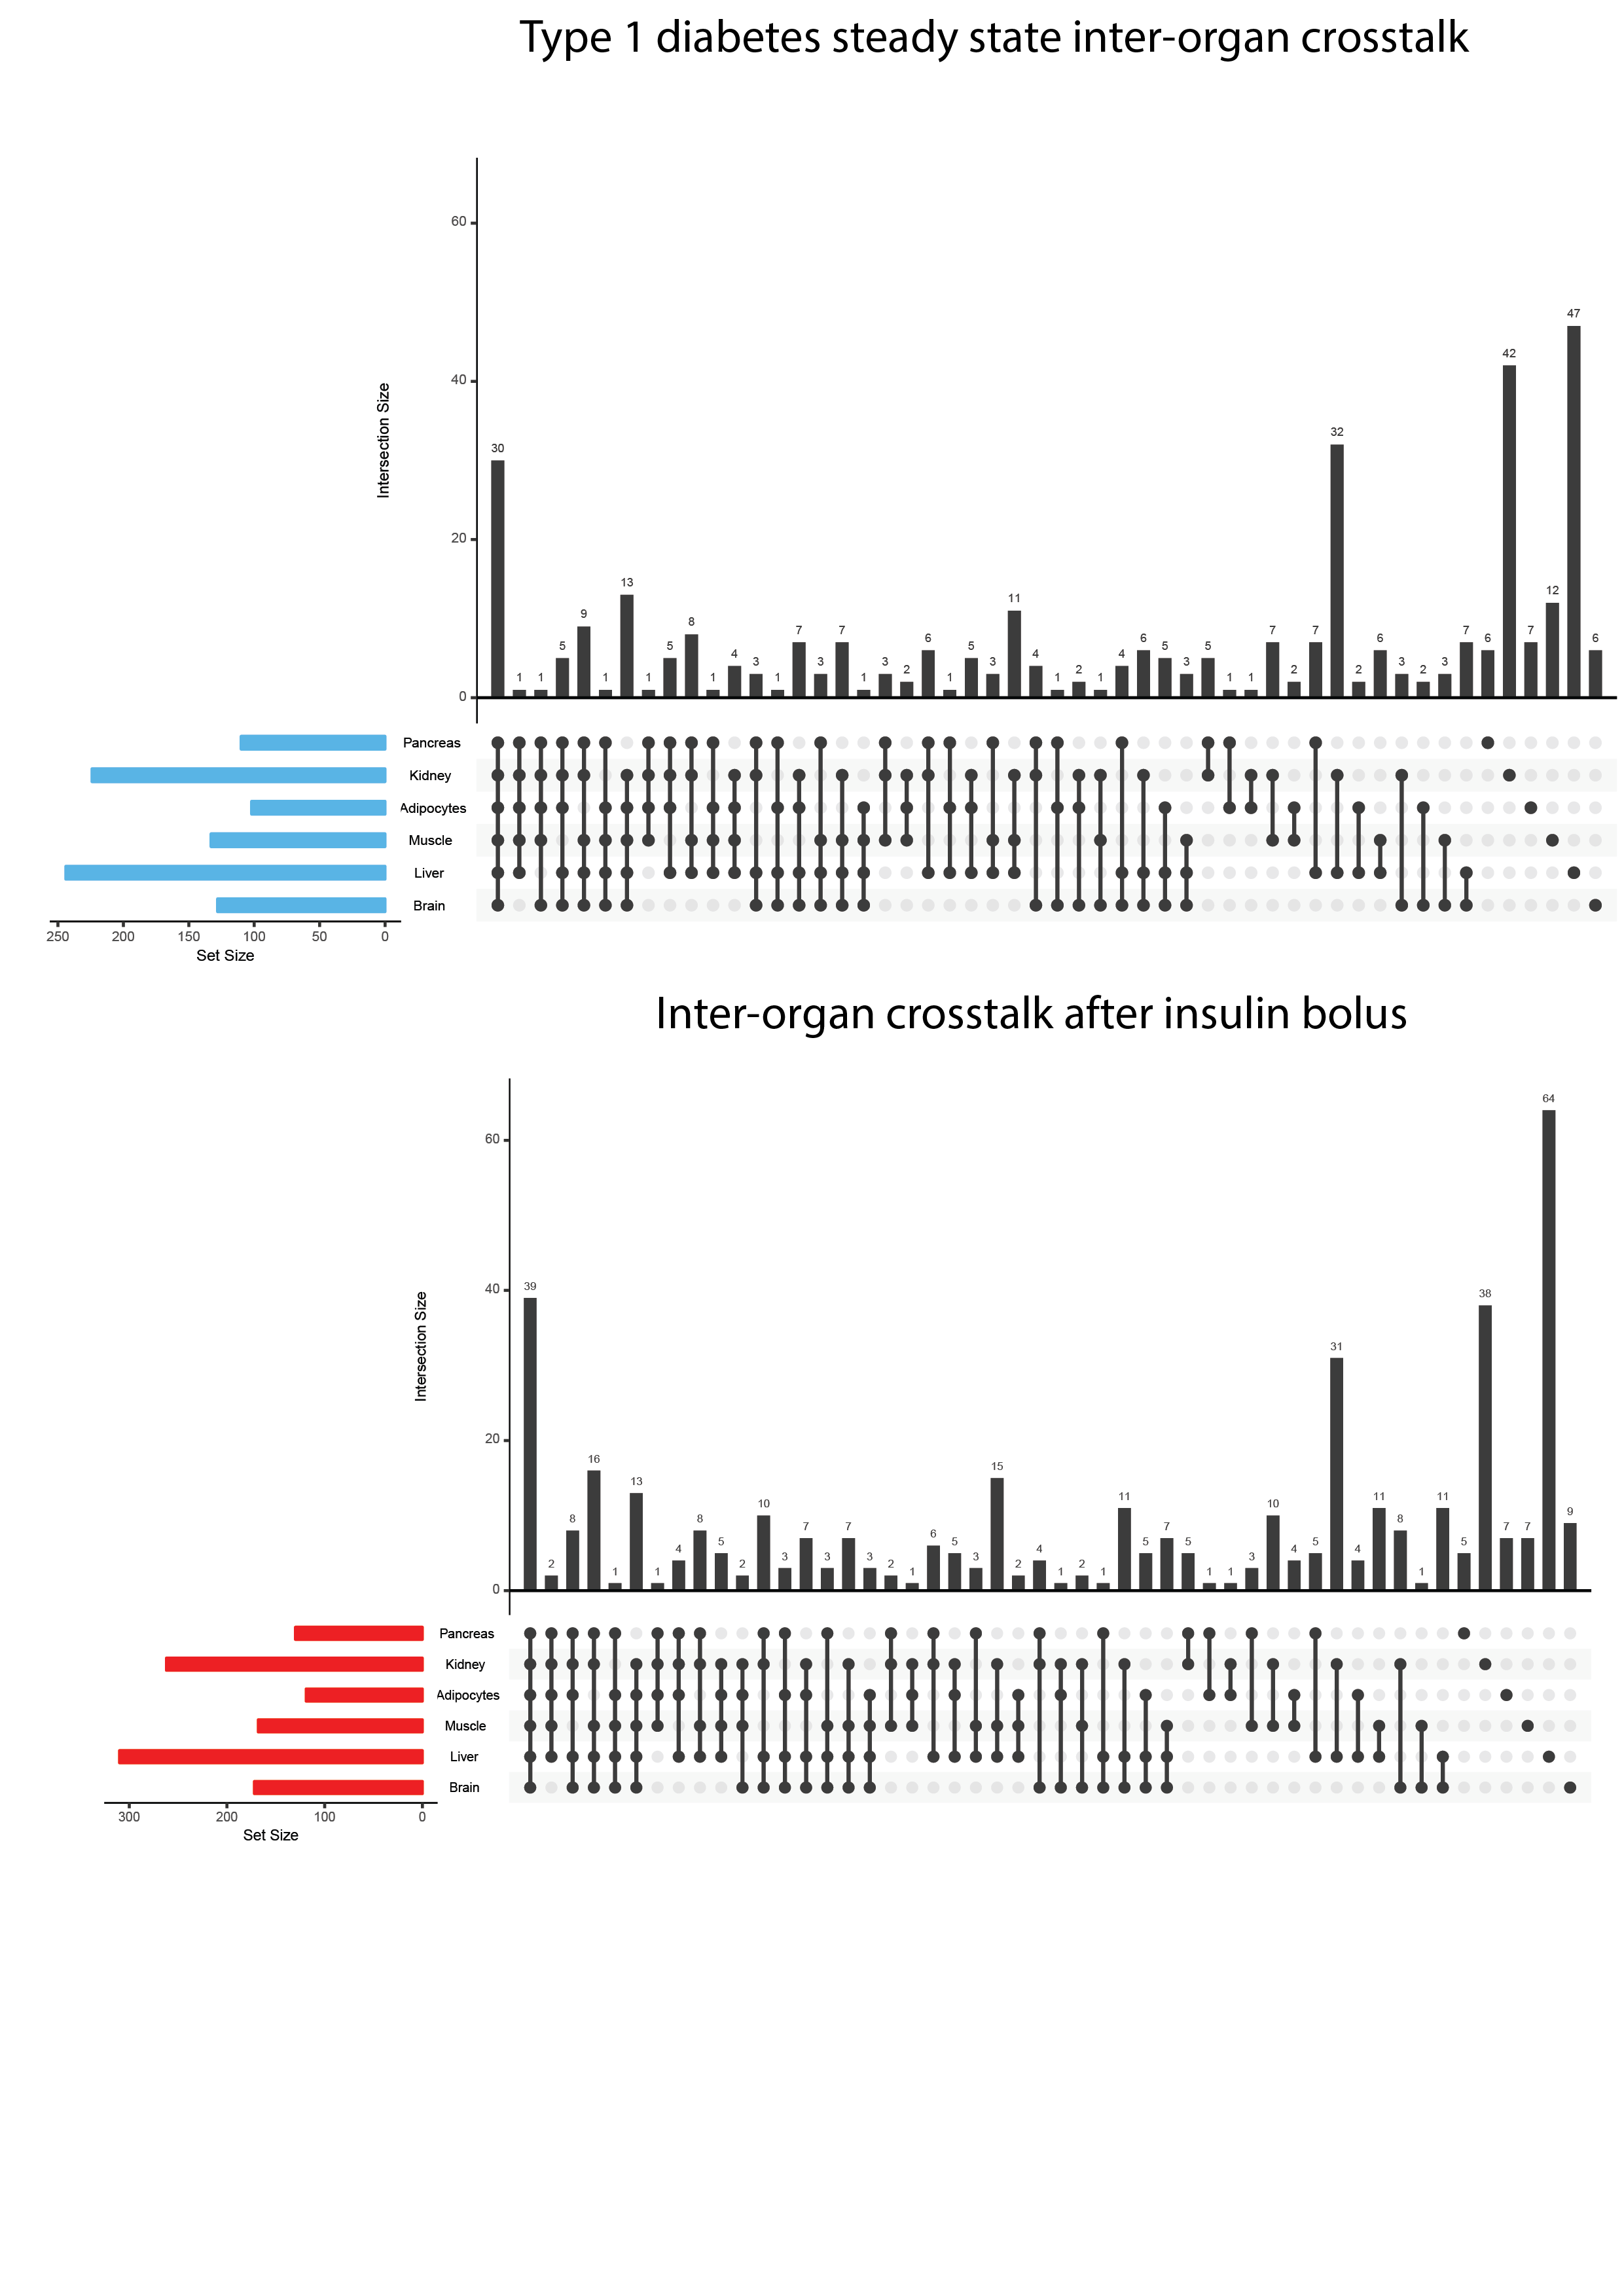
\includegraphics[width=\textwidth,height=\textheight,keepaspectratio]{GIM/figure3c.png}%Figure from images\Figure1.png
	\caption[Insulin induced inter-organ cross-talk.]{Pancreas, kidney, adipocytes, muscle, liver, and brain metabolic crosstalk with and without insulin action.}
	\label{fig:GIM3c}
\end{figure}


\begin{figure}[!htp]
\centering
	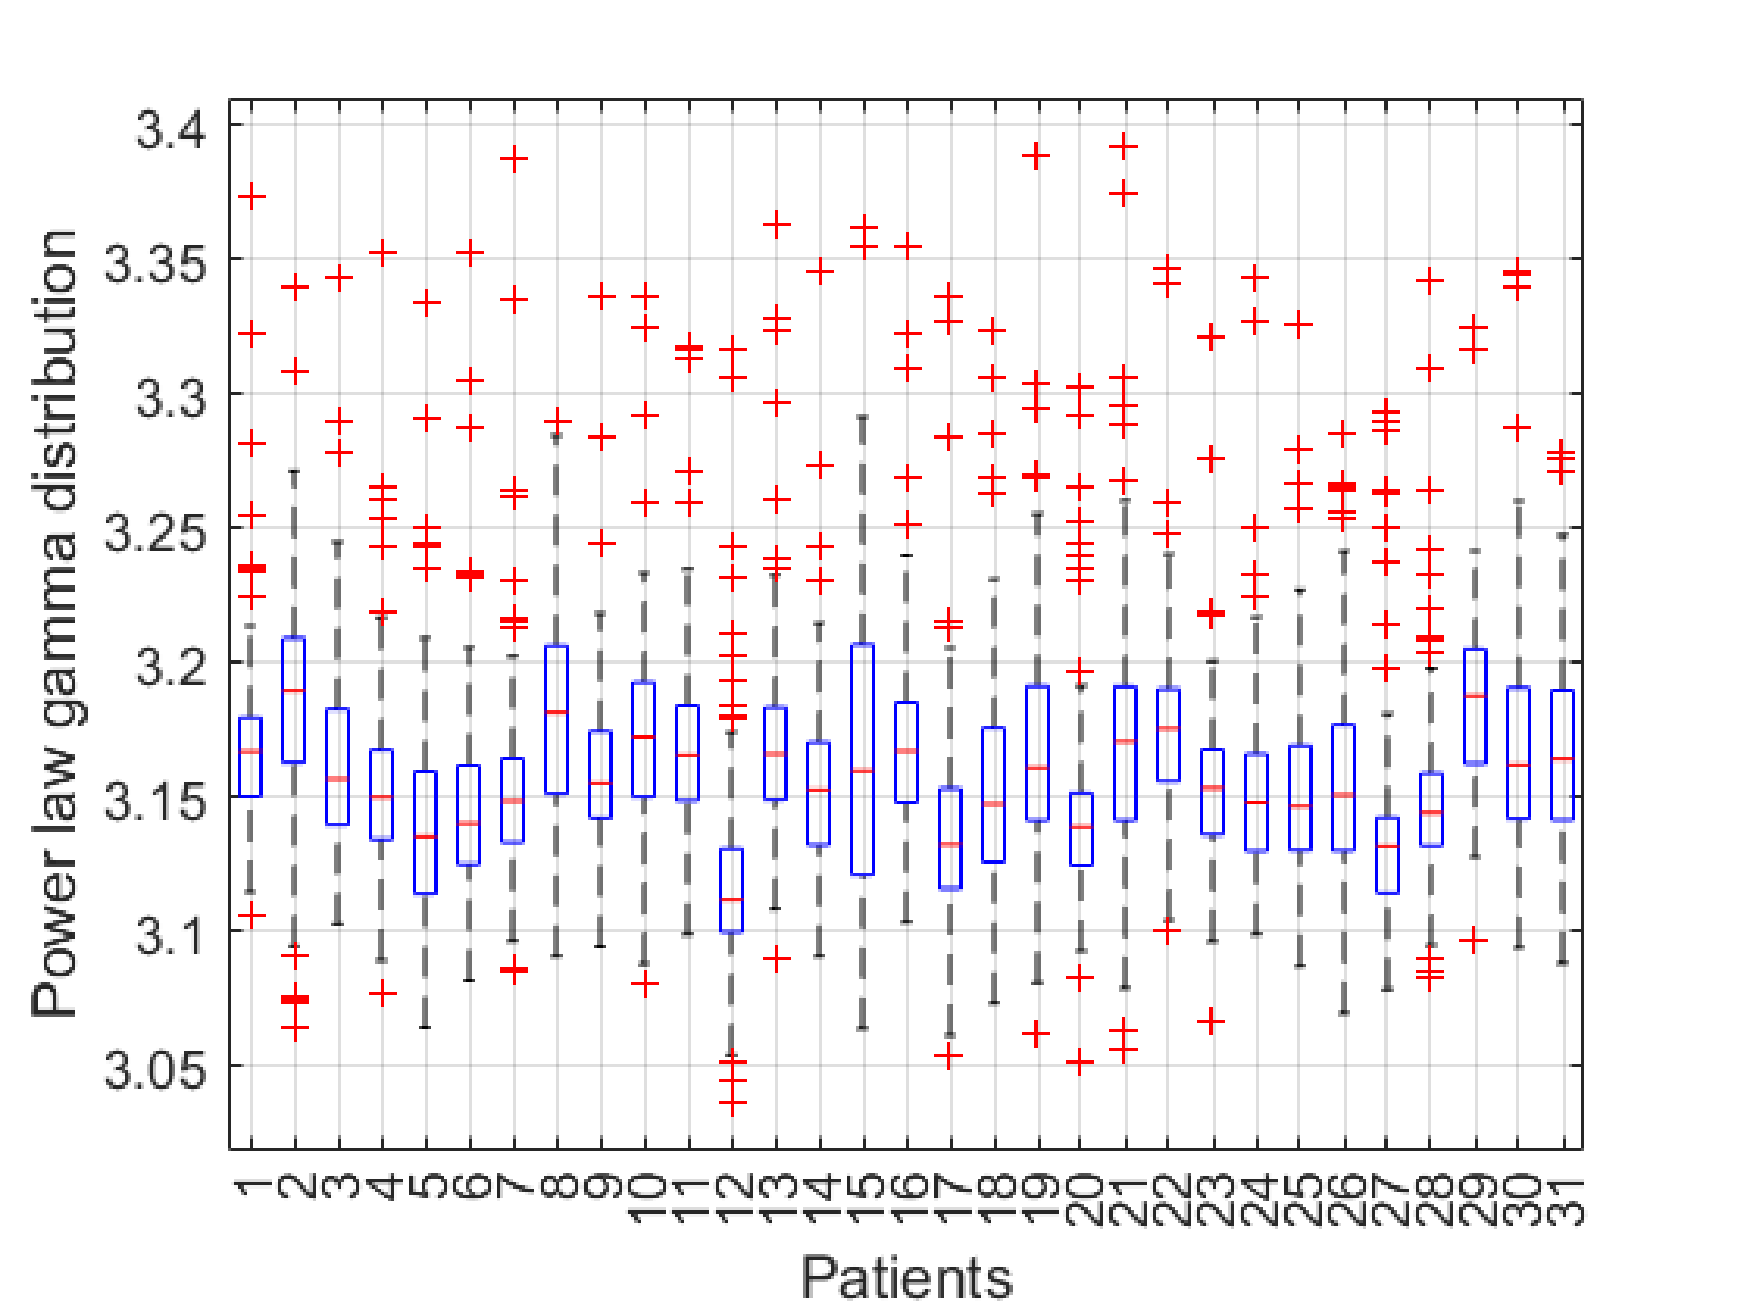
\includegraphics[width=\textwidth,height=\textheight,keepaspectratio]{GIM/figureS4.png}%Figure from images\Figure1.png
	\caption[Variation of the power law gamma across patients after a subcuetanous insulin injection.]{Variation of the power law gamma across patients after a subcutaneous insulin injection. For every patient, the changes of the metabolic network topology were assessed through fitting the metabolite-centric model connectivity on a power law. The variation of the gamma parameter during the simulation time was represented in the boxplot. Overall, the network structure is quite stable across patients and the gamma parameter mean value stays between 3.1 and 3.2 as reported for biological networks \cite{ravasz2002hierarchical}.}
	\label{fig:s4GIM}
\end{figure}

\begin{table}[h]
\caption[Selected metabolic reactions with the highest sensitivities towards peripheral glucose concentrations.]{Selected metabolic reactions with the highest sensitivities towards peripheral glucose concentrations. Type refers to interface reactions (I) shared by Harvey and GIM, and (H) for the reactions belonging to Harvey alone. The letters in brackets refer to the cellular compartments, where e is exrtacellular, c for cytoplasm, m for mitochondria, n for nucleus, and r for endoplasmic reticulum}
\begin{center}
	\begin{tabular*}{\textwidth}{l @{\extracolsep{\fill}} ll}
	\hline
	Name/Type  & Reaction & Subsystem       \\ 
	\hline
	Glut4(I)                   & na1[e]+glc\_D[e] $\leftrightarrow$ na1[c]+glc\_D[c] & Transport      \\
	NMNATr(H)                      & atp[c]+h[c]+nmn[c] $\leftrightarrow$ nad[c]+ppi[c] & NAD metabolism         \\
	GF6PTA(H)            			& f6p[c]+ gln\_L[c] $\rightarrow$ gam6p[c]+glu\_L[c] & Aminosugar metabolism         \\
	TRPO2(H)             			& o2[c]+trp\_L[c] $\rightarrow$ Lfmkynr[c] & Tryptophan metabolism        \\
    HMR\_1280(H)          			& CE4988[c]+nadp[c] $\leftrightarrow$  & Leukotriene metabolism       \\
    & CE5944[c]+h[c]+nadph[c] &\\
	SPODMm(H)            			& 2 h[m]+ 2 o2s[m] $\rightarrow$ h2o2[m]+o2[m] & ROS detoxification        \\
	GUAPRT(H)            			& gua[c]+prpp[c] $\rightarrow$ gmp[c]+ppi[c] & Nucleotide salvage pathway        \\
	DTMPKm(H)            			& atp[m]+dtmp[m] $\rightarrow$ adp[m]+dtdp[m] & Pyrimidine synthesis        \\
	PPNCL3(H)           			& 4ppan[c]+atp[c]+cys\_L[c] $\rightarrow$  & CoA synthesis      \\
	                                & 4ppcys[c]+amp[c]+h[c]+ppi[c]             & \\
	GGT\_L(H)             			& 17.6 ipdp[c]+ttc\_ggdp[c] $\rightarrow$ & N-glycan synthesis        \\
	                                &  0.1 dedoldp\_L[c] + 17.6 ppi[c] & \\
	EX\_ha(e)(H)          			& ha[e] $\leftrightarrow$ & Exchange/demand reaction       \\
	r0301(H)             			& atp[c]+nh4[c]+xmp[c] $\rightarrow$ & Bile acid synthesis        \\
	                                & amp[c]+gmp[c]+2 h[c]+ppi[c] & \\
	PAN4PP(H)            			& h2o[c]+pan4p[c]$\rightarrow$ pi[c]+ptth[c] & CoA catabolism       \\
	RE2235R(H)           			& estrone[r]+h[r]+nadph[r]+o2[r] $\rightarrow$ & Androgen and estrogen        \\
	                                &  C05300[r]+h2o[r]+nadp[r]                    & synthesis and metabolism \\
	IPDDI(H)             			& ipdp[c] $\leftrightarrow$ dmpp[c] & Squalene and cholesterol         \\
	 & &  synthesis\\
	DASCBR(H)            			& dhdascb[c]+nadph[c] $\rightarrow$ ascb\_L[c]+nadp[c] & Vitamin C metabolism        \\
	r0009(H)             			& h2o[x]+ppi[x] $\rightarrow$ h[x]+2 pi[x] & Purine metabolism      \\
	SBTR(H)             			& glc\_D[c]+h[c]+nadph[c] $\rightarrow$ nadp[c]+sbt\_D[c] & Fructose and mannose         \\
	& & metabolism\\
	RE1303C(H)           			& h[c]+nadph[c]+o2[c]+vitd3[c] $\rightarrow$   & Vitamin D metabolism      \\
	                                & 25hvitd3[c] + h2o[c] + nadp[c]               &\\
	r2073(H)             			& h[e]+zn2[e] $\rightarrow$ h[c]+zn2[c] & Transport, extracellular        \\
	EX\_icdchol(H)        			& icdchol[e] $\leftrightarrow$ & Exchange/demand reaction       \\
	EX\_CE2934(e)(H)      			& CE2934[e] $\leftrightarrow$ & Exchange/demand reaction        \\
	P4507A1r(H)          			& chsterol[r]+h[r]+nadph[r]+o2[r] $\rightarrow$ & Bile acid synthesis        \\
	                                & h2o[r]+nadp[r]+xol7a[r] & \\
	RAtn3(H)             			& 13\_cis\_retn[c] $\leftrightarrow$ 13\_cis\_retn[n] & Transport, nuclear       \\
	\hline
	\end{tabular*}
\end{center}
\label{GIM:tblsRxn}%descriptive label to refer to figure in text
\end{table}